% !Rnw root = learnR.Rnw






\marginnote{The function \margtt{plot()} accepts a \margtt{data} argument,
while \margtt{lines()}, \margtt{points()} and \margtt{text()} do not.}
\noindent
\fbox{\parbox{\textwidth}{{\bf Base Graphics (mostly 2-D):}\\[4pt]
\begin{tabular}{ll}
\multicolumn{2}{l}{Base graphics implements a ``traditional'' style
of graphics}\\[0.15cm]
Functions & \txtt{plot()}, \txtt{points()}, \txtt{lines()},
  \txtt{text()}, \\
&  \txtt{mtext()}, \txtt{axis()},\txtt{identify()} etc. form\\
& a suite that plot points, lines, text, etc.\\[6pt]
\end{tabular}
}}
\vspace*{4pt}

\marginnote[27pt]{{\em lattice} and {\em ggplot2} are built on the low-level
  graphics package {\em grid}.

Note also various special types of graph.  For example
word clouds, as in the {\em wordcloud} package, list words
with size proportional to frequency.}
\noindent
\fbox{\parbox{\textwidth}{
{\bf Other Graphics}\\[4pt]
\begin{tabular}{ll}
  \multicolumn{2}{l}{\quad (i) lattice (trellis) graphics, using the
    \textit{lattice} package,}\\
  \multicolumn{2}{l}{\quad (ii) \textit{ggplot2}, implementing Wilkinson's
    \textit{Grammar} \textit{of Graphics}}\\
  \multicolumn{2}{l}{\quad (iii) For 3-D graphics (Section
    \ref{sec:dynamicg}), note \textit{rgl}, \textit{misc3d} \&
    \textit{tkrplot}}\\
  \multicolumn{2}{l}{\quad (iv) \textit{Motion Charts} (Section
\ref{sec:gvis}), show a scatterplot changing}\\
 & with movement forward or backward in time.\\
\end{tabular}
}}
\vspace*{18pt}

Consider first base graphics.  Relative to {\em lattice} and to {\em
  ggplot2}, the more traditional style of base graphics is less
consistent and less structured.  Each system however has its own
strengths and uses.

\begin{Schunk}
\begin{Sinput}
## DAAG has several datasets that will be required
library(DAAG, quietly=TRUE)
\end{Sinput}
\end{Schunk}

\section{Base Graphics}\label{sec:baseplots}

\begin{marginfigure}
  To see a variety of base (or traditional) graphics plots, enter\\[-4pt]
\begin{Schunk}
\begin{Sinput}
demo(graphics)
\end{Sinput}
\end{Schunk}
\noindent Press Enter to see each new graph.
\end{marginfigure}

The function \txtt{plot()} is the most basic of several functions that
create an initial graph. Other functions can be used to add to an
existing graph. Note in particular \txtt{points()} \txtt{lines()} and
\txtt{text()}.

\subsection{\txtt{plot()} and allied base graphics functions}
The following are alternative ways to plot \txtt{y} against \txtt{x}
(obviously \txtt{x} and \txtt{y} must be the same length):

\begin{marginfigure}[-3pt]
Plot \margtt{height} vs \margtt{weight} --\\
\begin{Schunk}
\begin{Sinput}
## Older syntax:
with(women,
     plot(height, weight))
\end{Sinput}
\end{Schunk}
\begin{Schunk}
\begin{Sinput}
## Graphics formula:
plot(weight ~ height,
     data=women)
\end{Sinput}
\end{Schunk}
\end{marginfigure}
\begin{Schunk}
\begin{Sinput}
plot(y ~ x)   # Use a formula to specify the graph
plot(x, y)    # Horizontal ordinate, then vertical
\end{Sinput}
\end{Schunk}

The following use the argument \txtt{data} to supply the name of a
data frame whose column names appear in the graphics formula:
\begin{Schunk}
\begin{Sinput}
plot(distance ~ stretch, data=elasticband)
plot(ACT ~ year, data=austpop, type="l")
plot(ACT ~ year, data=austpop, type="b")
\end{Sinput}
\end{Schunk}

The \txtt{points()} function adds points, while \txtt{lines()} adds
lines\footnote{These functions differ only in the default
  setting for the parameter \txtt{type}{\small .}  Explicitly setting
\txtt{type = "p"} causes either function to plot points.}  to a plot.
The \txtt{text()} function adds text at specified locations.  The
\txtt{mtext()} function places text in one of the margins.  The
\txtt{axis()} function gives fine control over axis ticks and labels.

Here is a further possibility
\begin{Schunk}
\begin{Sinput}
with(austpop, plot(spline(year, ACT), type="l"))
  # Fit smooth curve through points
\end{Sinput}
\end{Schunk}

\subsection*{Adding text -- an example}\label{ss:addpoints}
Here is a simple example (Figure \ref{fig:primates}) that uses the
function \txtt{text()} to label the points on a plot. Data is from
the dataset \txtt{primates} ({\em DAAG}).  The first two lines of
data are:
\begin{Schunk}
\begin{Sinput}
## Data (1st 2 lines)
head(primates, 2)
\end{Sinput}
\begin{Soutput}
             Bodywt Brainwt
Potar monkey     10     115
Gorilla         207     406
\end{Soutput}
\end{Schunk}

\begin{marginfigure}
\begin{Schunk}


\centerline{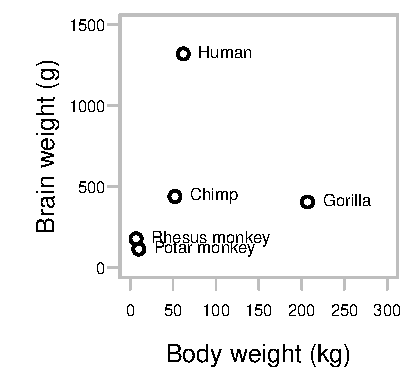
\includegraphics[width=\textwidth]{figs/09-brain-body-1} }

\end{Schunk}
\caption{Plot of brain weight against body weight, for selected
primates.
}\label{fig:primates}
\end{marginfigure}

Code for a simplified version of the plot is:
\begin{Schunk}
\begin{Sinput}
plot(Brainwt ~ Bodywt, xlim=c(0, 300),
     ylim=c(0,1500), data=primates, fg="gray",
     xlab="Body weight (kg)",
     ylab="Brain weight (g)")
# Specify xlim to allow room for the labels
with(primates,
     text(Brainwt ~ Bodywt, cex=0.8,
          labels=rownames(primates), pos=4))
# pos: pos=1 (below), 2 (left), 3 (above)
\end{Sinput}
\end{Schunk}

\subsection*{Identification and Location on the Figure Region}
Draw the graph first, then call the required function.
\marginnote{Section \ref{ss:shortR} described how to
terminate the plot, if the limit \txtt{n} is not reached first.
For \txtt{locator()}, \txtt{n} is by default set to 500.}
\begin{itemizz}
\item[-] \txtt{identify()}, discussed in Subsection \ref{ss:shortR}, labels
points.
\item[-] \txtt{locator()} prints out the co-ordinates of
points. Position the cursor at the location for which coordinates are
required, and click the left mouse button.
\end{itemizz}

\subsection{Fine control -- Parameter settings}\label{ss:fine}
\begin{marginfigure}[24pt]
  To store existing settings for later restoration, proceed thus:
\begin{Schunk}
\begin{Sinput}
oldpar <- par(cex=1.25)
  # par(oldpar) to restore
\end{Sinput}
\end{Schunk}
\end{marginfigure}
In most (not all) instances, parameters can be set either using
\txtt{par()}, or in a call to a plotting function (\txtt{plot()},
\txtt{points()}, \ldots).  Changes made using \txtt{par()} remain in
place until changed again, or until a new device is opened.  If made
in a call to a plotting function, the change applies only to that
call.

Some of the more common settings are:\\[-3pt]
\begin{itemize}
\item[-] Plotting symbols: \verb+pch+ (choice of symbol); \verb+cex+
  ("character expansion")\sidenote{Thus \texttt{par(cex=1.2)}
    increases plot symbol size 20\% above the default.}; \verb+col+
  (color).
\item[-] Lines: \verb+lty+ (line type); \verb+lwd+ (line width); \verb+col+
(color).
\item[-] Axis limits: \verb!xlim!; \verb!ylim!.
\item[-] Closeness of fit to the axis limits: \txtt{xaxs},
  \txtt{yaxs}.\sidenote{The default is \txtt{xaxs="r"}; $x$-axis limits are
extended by 4\% relative to data or \txtt{xlim} limits.} Specify
  \txtt{xaxs="i"} for an exact fit to the data limits.
\item[-] Axis annotation and labels: \verb+cex.axis+ (for axis
  annotation, independently of \verb+cex+);
  \verb+cex.labels+ (for axis labels).
\item[-] Margins and positioning within
  margin:\sidenote{Parameters such as \txtt{mar}, \txtt{mgp} and
    \txtt{oma} specify distances in `lines' out from the relevant
    boundary of the figure region. Lines are in units of \txtt{mex},
    where by default \txtt{mex=1}.}  \verb+mar+ (inner margins
  clockwise from bottom, out of box default \txtt{mar=c(5.1, 4.1, 4.1,
    2.1)}); \verb+oma+ (outer margins, use when there are multiple
  plots on the one graphics page); positioning within margin:
  \verb+mgp+ (margin line for the axis title, axis labels, and axis
  line, default \txtt{mgp=c(3, 1, 0)}).
 \item[-] Plot shape: \txtt{pty="s"} gives a square
plot.\sidenote{This must be set using \txtt{par()}}
(default is \txtt{pty="m"})
\item[-] Multiple graphs on the one graphics page: \marginnote{For a 1
    by 2 layout of plots; specify \txtt{par(mfrow=c(1,2))}.
    Subsection \ref{ss:sum-modobj} has an example.} \txtt{par(mfrow=c(m,n))}
  gives an $m$
  rows by $n$ columns layout.
\end{itemize}
Type \txtt{help(par)} to get a (very extensive) complete list.  Figure
\ref{fig:pars} demonstrates some of the possibilities.

\subsection{Color and Opacity}

The function \txtt{colors()} gives access to 657 different color names,
some of them repeats of the same colour. The function \texttt{palette()}
can be used to show or set colors that will by default be used for base
graphics.  Thus
\begin{itemizz}
  \item[-] \txtt{palette()} lists the colors in the current palette;
  \item[-] as an example, \txtt{palette(rainbow(6))} sets the current
    palette to a 6-color rainbow palette;
  \item[-] \txtt{palette("default")} resets back to the default.
\end{itemizz}

\marginnote[12pt]{See \txtt{help(palette)} for palettes in the base R
  {\em grDevices} package.}  Run the following code to show the
default palette, three sequential palettes from {\em grDevices}, a
color ramp palette given by the function \txtt{colorRampPalette()},
and two quantitative palettes from the {\em RColorBrewer} package.

\begin{fullwidth}
\begin{Schunk}
\begin{Sinput}
## Load to run code for Supplementary Figure 1
library(RColorBrewer)   # Required for Set1 and Dark2 RColorBrewer palettes
\end{Sinput}
\end{Schunk}

\begin{Schunk}
\begin{Sinput}
colpal <- rev(list(
    "Default palette" = palette()[1:8],  cm.colors = cm.colors(12),
    terrain.colors = terrain.colors(12), heat.colors = heat.colors(12),
    blueRamp = colorRampPalette(c(blues9, "white"))(12),
    "Brewer-Set1" = brewer.pal(8, "Set1"),
    "Brewer-Dark2" = brewer.pal(8, "Dark2")))
palnam <- names(colpal)
plot(1, 1, xlim=c(0.5,12.5), ylim=c(0,length(palnam)+0.5), type="n",
     axes=FALSE, xlab="", ylab="")
for(i in 1:length(palnam)){
    len <- length(colpal[[i]])
    points(1:len, rep(i,len), pch=15, col=colpal[[i]], cex=5.5)
    legend(1, i+0.025, palnam[i], adj=0, box.col="white", bg="white",
           x.intersp=0, y.intersp=0, yjust=0)
\end{Sinput}
\end{Schunk}
\end{fullwidth}
Each of these palettes, except the default, allows variation in the
number of colors, up to a maximum.  The palettes available from {\em
  RColorBrewer} include other qualitative palettes, sequential
palettes, and diverging (light in the middle; dark at the extremes)
palettes.  To see the full range of {\em RColorBrewer} possibilities,
type: \marginnote{Stretch the graphics window vertically (pull on an
  edge) so that rows do not overlap.}
\begin{Schunk}
\begin{Sinput}
display.brewer.all()
\end{Sinput}
\end{Schunk}
\noindent
\marginnote{While limited use of light colors is fine for
  coloring regions on a map, light colors do not show up well
  when coloring points on a graph.}  Qualitative schemes that may be
suited for use in plots are "Set1" with yellow (the 6$^{th}$ color out
of nine) omitted, or "Dark2", or "Accent" with the 4$^{th}$ color
(out of 8) omitted.  To extract these, do for example:
\begin{Schunk}
\begin{Sinput}
Set1 <- brewer.pal(8, "Set1")[-6]
## Check out the palette
plot(1:7, pch=16, cex=2, col=Set1)
\end{Sinput}
\end{Schunk}

\subsection*{Opacity, and graphs with many points}\label{ss:xpoint}

\begin{figure}
\begin{Schunk}


\centerline{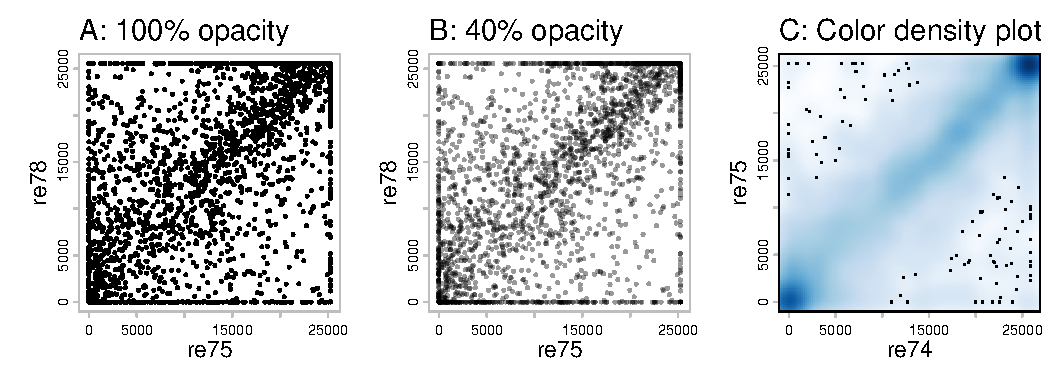
\includegraphics[width=\textwidth]{figs/09-alpha-ex-1} }

\end{Schunk}
\caption{In Panel A, points are plotted with the 100\% opacity, i.e.,
  no transparency. In Panel B, \txtt{alpha=0.4}, i.e., 40\% opacity.
  Panel C uses the function \txtt{smoothScatter()} to show a smoothed
  color density representation of the data.  Figure \ref{col:alphaC}
  is a color version of Panel C.\label{fig:alpha}}
\end{figure}

\marginnote[2pt]{An opacity of 0.4 has the effect that, for an
  isolated point, 60\% of the white background shows through.}
\noindent
\begin{Schunk}
\begin{Sinput}
## Sample from the 15992 rows
dfsamp <- cps1[sample(nrow(cps1), 3000), ]
plot(re78 ~ re75, data=dfsamp, pch=20, cex=0.5,
     col="black", fg="gray")
mtext(side=3, line=0.5, "A: 100% opacity", adj=0)
plot(re78 ~ re75, data=dfsamp, pch=20, cex=0.5,
     col=adjustcolor("black", alpha=0.4), fg="gray")
mtext(side=3, line=0.5, "B: 40% opacity", adj=0)
blueRamp <- colorRampPalette(c("white", blues9))
with(dfsamp, smoothScatter(re75~re74, , fg="gray",
                           colramp=blueRamp))
mtext(side=3, line=0.5, "C: Color density plot",
      adj=0)
\end{Sinput}
\end{Schunk}
With \txtt{alpha=0.4}, two overlapping points have a combined
opacity of 80\%, so that 20\% of the white background shows through.
Three or more overlapping points appear as completely black.

\marginnote[11pt]{The plots show a sample of 3000 of the
  points.  Plotting all the points gives an incoveniently large
  graphics file, while not giving a more informative graph.}  Compare
three plots shown in Figure \ref{fig:alpha}.  Points overlap to such
an extent that Panel A, gives very limited information about the
density of points.  Panel B, where the color opacity is 40\%, gives a
better indication of variation in the density of points.  Panel C uses
the function \txtt{smoothScatter()} to provide a color density
representation of the scatterplot.  This is a more nuanced
way to show the density of points.

\subsection{The shape of the graph sheet}
Aspect ratio, i.e., the ratio of $x$-distance to $y$-distance, has a
large say in what is visually obvious.  Figures \ref{fig:aspect}A and
\ref{fig:aspect}B show the same data:
\begin{figure*}
\begin{Schunk}


\centerline{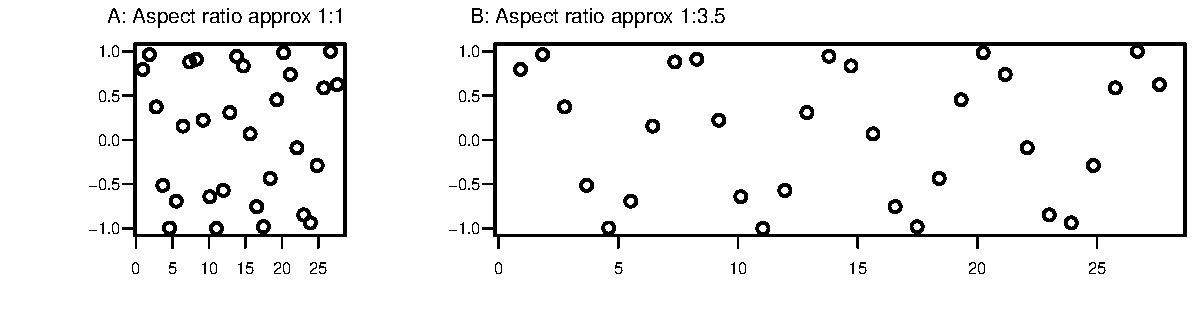
\includegraphics[width=\textwidth]{figs/09-fig8_3e-1} }

\end{Schunk}
\caption[][-15pt]{Figures A and B show the same data, but with widely different
  aspect ratios.\label{fig:aspect}}
\end{figure*}
\noindent
Features that are at an angle that is close to the horizontal or the
vertical are hard to detect visually. Patterns of change or other
features should, to be visually obvious, be offset by an angle of
at least 20$^\circ$ from both the horizontal and the vertical.

\noindent For each of Figures \ref{fig:aspect}A and \ref{fig:aspect}B
the code, after setting the dimensions of the figure page, is:
\begin{Schunk}
\begin{Sinput}
plot((1:30)*0.92, sin((1:30)*0.92),
     xlab="", ylab="")
\end{Sinput}
\end{Schunk}

The dimensions of the graphics display can be specified when a
graphics window is opened.  Once opened, the shape and size of a
screen device can be changed by clicking and dragging on one corner.

The R for Windows functions \txtt{win.graph()} or \txtt{x11()} that
set up the Windows screen take the parameters \txtt{width} (in
inches), \txtt{height} (in inches) and \txtt{pointsize} (in 1/72 of an
inch). The setting of \txtt{pointsize} (default =12) determines
character heights. It is the relative sizes that matter for screen
display or for incorporation into Word and similar programs.

\subsection{Multiple plots on the one page}\label{ss:xplots}
\marginnote[10pt]{For a layout in which columns are filled before
  moving to a new row, use \margtt{mfcol} in place
  of \margtt{mfrow}.}
The parameter \txtt{mfrow} can be used to configure the graphics
sheet so that subsequent plots appear row by row, one after the
other in a rectangular layout, on the one page. The following
presents four different transformations of data from the dataset
\txtt{Animals} ({\em MASS}),
in a two by two layout:
\begin{Schunk}
\begin{Sinput}
## Supplementary figure 9.2
library(MASS)
oldpar <- par(pch=16, pty="s", mfrow=c(2,2))
with(Animals, {      # bracket several R statements
  plot(body, brain)
  plot(sqrt(body), sqrt(brain))
  plot(body^0.1, brain^0.1)
  plot(log(body), log(brain))
})                   # close both sets of brackets
par(oldpar)          # Restore former settings
\end{Sinput}
\end{Schunk}

A more flexible alternative is to use the graphics parameter
\txtt{fig} to mark out the part of the graphics page on which the
next graph will appear.  The following marks out, successively,
a plot region that occupies the upper 62\% of the plot region,
then the lower 38\%.
\marginnote[15pt]{\margtt{par(fig = c(0,1,0.38,1))} marks out a
  plot region that is the total width, starts
  38\% of the way up, and extends to the top.
  \margtt{par(fig=c(0,1,0,0.38), new=TRUE)} marks out the lower
  38\% of the page.}
\begin{Schunk}
\begin{Sinput}
par(fig = c(0, 1, 0.38, 1))
          # xleft, xright, ybottom, ytop
## Panel A
par(fig = c(0, 1, 0, 0.38), new=TRUE)
## Plot graph B
par(fig = c(0, 1, 0, 1))    # Restore settings
\end{Sinput}
\end{Schunk}
The effect of \txtt{new=TRUE} is, somewhat
counter-intuitively, ``assume a new page is already open; do not open
a new page''.

\subsection{Plots that show the distribution of data values}
\marginnote{Density plots are much preferable, for most purposes, to
  histograms.  Both have limitations.}  We discuss
histograms, density plots, boxplots and normal probability plots.
Normal probability plots are a specialised form of cumulative
density plot.

\subsection*{Histograms and density plots}
\begin{figure}[htbp]
\begin{Schunk}


\centerline{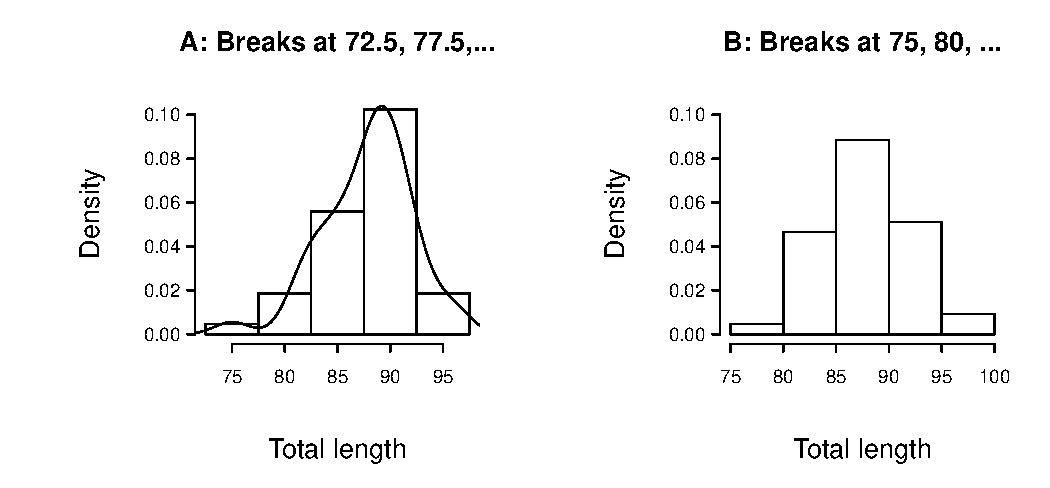
\includegraphics[width=\textwidth]{figs/09-poss-hist-1} }

\end{Schunk}
 \caption{The two panels show the same data, but with a different
choice of breakpoints.\label{fig:densitybreaks}}
\vspace*{-15pt}
\end{figure}

The shapes of histograms depend on the placement of the breaks, as
illustrated by Figure \ref{fig:densitybreaks}.  The following code
plots the histograms and superimposes the density plots.
\marginnote[12pt]{The argument \txtt{freq=FALSE} gives a vertical
  scale that is the number of points per unit interval, i.e., it is
  the ``density'' estimate that is given by the upper bar of each
  rectangle.  This is needed for the superposition of a density curve
  onto the histogram.}
\begin{Schunk}
\begin{Sinput}
ftotlen <- subset(possum, sex=="f")[, "totlngth"]
## Left panel: breaks at 72.5, 77.5,..
hist(ftotlen, breaks = 72.5 + (0:5)*5, freq=FALSE,
     xlab="Total length", ylim=c(0,0.11),
     main ="A: Breaks at 72.5, 77.5,...")
## Now superimpose a density curve, as in Fig. 7.3
lines(density(ftotlen))
##
## Panel B: breaks at 75, 80, ...
hist(ftotlen, breaks = 75 + (0:5)*5, freq=FALSE,
     xlab="Total length", ylim=c(0,0.11),
     main="B: Breaks at 75, 80, ...")
\end{Sinput}
\end{Schunk}

The height of each rectangle of a histogram provides a crude density
estimate. These estimates change in jumps, at breakpoints that are
inevitably chosen somewhat arbitrarily.
A smoothly changing density estimate, such as given by the
superimposed density curves in the panels of Figure
\ref{fig:densitybreaks}, makes better sense than an estimate that
changes in jumps.

\marginnote[12pt]{Neither histograms nor density plots are effective
  for checking normality.  For that, use a normal probability plot.}
Unless samples are very large, the shape of both histograms and
density plots will show large statistical variability.  Density plots
are helpful for showing the mode, i.e., the density maximum.

The following gives a density plot, separately from the histograms that
are shown in \ref{fig:densitybreaks}.
\begin{Schunk}
\begin{Sinput}
## Supplementary figure 9.3
with(subset(possum, sex=="f"),
     plot(density(totlngth), type="l"))
\end{Sinput}
\end{Schunk}

For use of density plots with data that have sharp lower and/or upper
cutoff limits, it may be necessary to specify the $x$-axis limit or
limits.\sidenote[][-18pt]{Thus, a failure time distribution will have a
  sharp cutoff at zero, which may also be the mode.} Use the
parameters \txtt{from} and/or \txtt{to} for this purpose. This issue
most commonly arises with a lower cutoff at 0.

\subsection*{Boxplots}

Boxplots use a small number of characteristics of a distribution to
characterize it. Look up \txtt{help(boxplot)} for details.
It can be insightful to add a ``rug'' that shows the individual values,
by default along the horizontal axis (\txtt{side=1}).
Figure \ref{fig:boxrugs} is an example.  Code for the plot is:
\begin{marginfigure}
\begin{Schunk}


\centerline{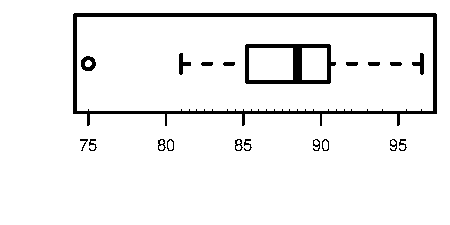
\includegraphics[width=\textwidth]{figs/09-boxplot-1} }

\end{Schunk}
\vspace*{-12pt}

\caption{Distribution of lengths of female possums.  The bars
  (together making up a 'rug') show actual data
  values.\label{fig:boxrugs}}
\end{marginfigure}

\begin{Schunk}
\begin{Sinput}
## Code
with(subset(possum, sex=="f"),
     {boxplot(totlngth, horizontal=TRUE)
      rug(totlngth)} )
\end{Sinput}
\end{Schunk}

The function \txtt{rug()} can be used to add, to any plot that shows a
distribution of data values, stubby vertical lines that show the
locations of the individual values.

\subsection*{Normal probability plots}

\marginnote{A point pattern that is not consistent with random deviation
  from a line indicates a non-normal distribution.}
The function \txtt{qqnorm(y)} gives a normal probability plot of the
values of \txtt{y}. In such a plot, data from a normal distribution
will be scattered about a line.  To calibrate the eye to recognise
plots that indicate non-normal variation, it helps to compare the plot
for the data in hand with several normal probability plots that use
\txtt{rnorm()} to generate random values.  Figure \ref{fig:np-plots}
is an example.

\begin{figure*}
\begin{Schunk}


\centerline{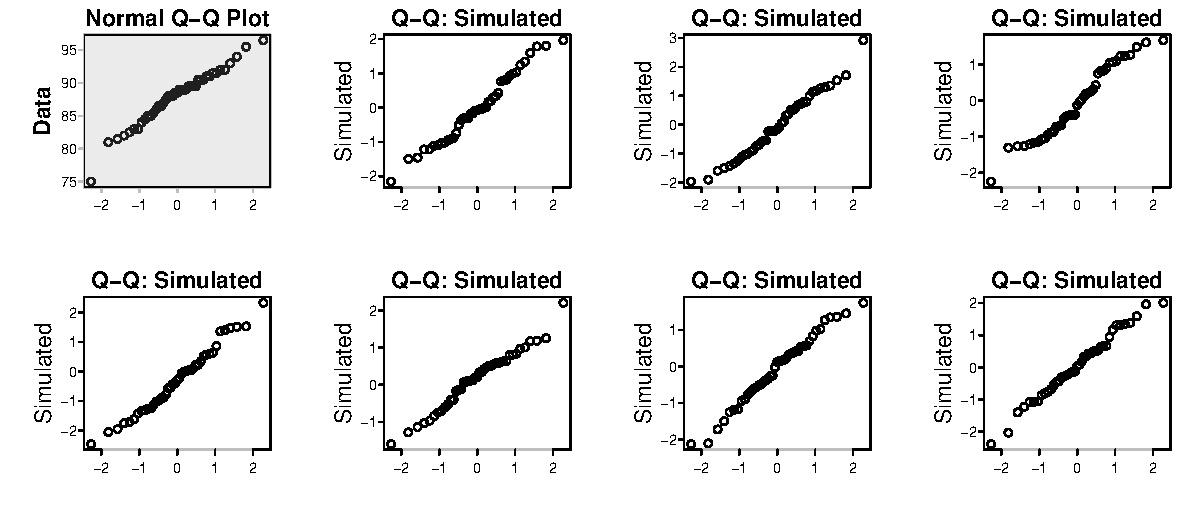
\includegraphics[width=\textwidth]{figs/09-possum-qqn-1} }

\end{Schunk}
 \caption[][7pt]{Normal probability plots. The top left panel
   shows the 43 lengths
of female possums. Other panels are for independent normal
random samples of size 43.\label{fig:np-plots}}
\vspace*{-24pt}

\end{figure*}

\begin{Schunk}
\begin{Sinput}
## Q-Q plot for the data (top left panel)
ftotlen <- subset(possum, sex == "f")[, "totlngth"]
qqnorm(ftotlen, xlab="",
       ylab=expression(bold("Data")))
## Code for a plot with random normal data
qqnorm(rnorm(43), xlab="", ylab="Simulated")
\end{Sinput}
\end{Schunk}

\noindent There is one unusually small value.  Otherwise the points
for the female possum lengths are as close to a straight line as in
many of the plots for random normal data.

\subsection{$^*$Plotting Text that Includes Technical  Symbols}\label{sec:mathvec}

\marginnote[11pt]{Axis labels can be expressions, in {\em lattice} and
  {\em ggplot2} as well as in base graphics.  Tick labels can for
  example be vectors of expressions.}
The functions \txtt{expression()} and {substitute()} can be used
to create mathematical expressions, for later evaluation or for
printing onto a graph.  For example, \verb+expression(x^2)+ will
print, when supplied to \txtt{text()} or \txtt{mtext()} or another
such function (this includes {\em lattice} and {\em ggplot2} functions),
as $x^2$.

For purposes of adding text that includes mathematical and other
technical symbols, the notion of expression is generalized, to allow
``expressions'' that it does not make sense to try to evaluate. For
example, \txtt{expression("Temperature (" * degree * "C)")} prints as:
$\mbox{Temperature (}^{\circ}\mbox{C)}$.
\marginnote[-22pt]{Items that are separated by an asterisk (\txtt{*})
  are juxtaposed side by side.  The initial text is followed by a
  degree symbol, and then by the final text.}

The following indicate some of the possibilities:
\begin{itemizz}
  \item[-] Letters such as \txtt{a}, \txtt{b}, \txtt{c}, \txtt{x},
    \ldots are printed literally.
  \item[-] \txtt{alpha} denotes the Greek letter $\alpha$, while
    \txtt{Alpha} denotes the upper case symbol.  Similarly for
    other Greek letters.
  \item[-] \txtt{hat(x)} denotes $\hat{\mbox{x}}$.
  \item[-] \txtt{italic(x)}, \txtt{bold(x)}, \txtt{bolditalic(x)},
    and \txtt{plain(x)} have the obvious meaning.
  \item[-] \txtt{frac(a,b)} denotes $\frac{\mbox{a}}{\mbox{b}}$.
 \end{itemizz}

Figure \ref{fig:area} demonstrates the use of an expression to
provide $y$-axis labeling.  The code is:
\begin{marginfigure}
\begin{Schunk}


\centerline{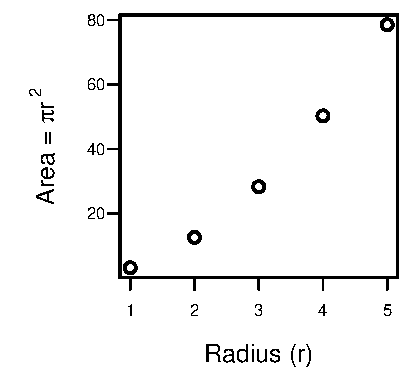
\includegraphics[width=\textwidth]{figs/09-plot-expr-1} }

\end{Schunk}
\caption{A mathematical expression is included as part of the
  $y$-axis label.\label{fig:area}.}
\end{marginfigure}
\begin{Schunk}
\begin{Sinput}
yl <- expression("Area = " * pi * r^~2)
plot(1:5, pi*(1:5)^2, xlab="Radius (r)", ylab=yl)
\end{Sinput}
\end{Schunk}
\noindent The tilde (\verb+~+) in \verb+r^~2+ is used to insert a small space.

Use \txtt{substitute()} in place of \txtt{expression()} when
symbols in the expression are to be replaced by values that
will be provided at the time of forming the expression.

See \txtt{help(plotmath)} for further details of the conventions,
and of the symbols that are available.  Type \txtt{demo(plotmath)}
to see a wide range of examples of what is possible.

\section{Lattice Graphics}
\marginnote[11pt]{The {\em lattice} package is included in all R binary
  distributions that are available from a CRAN (Comprehensive R
  Archive Network) mirror.  It implements a \textit{trellis} style of
  graphics, as in the S-PLUS implementation of the S language. It is
  built on the \textit{grid} low-level graphics system, described in
  Part II of Paul Murrell's \textit{R Graphics}}
\fbox{\parbox{\textwidth}{{\bf Lattice Graphics:}\\[4pt]
\begin{tabular}{ll}
\textbf{Lattice} & Lattice is a flavour of trellis graphics\\
 & (the S-PLUS flavour was the original)\\[6pt]
Lattice & Lattice is more structured, automated and stylized.\\
vs base & For standard purposes, much is automatic.\\[6pt]
Lattice  & Lattice syntax is consistent and tightly regulated\\
syntax & For lattice, graphics formulae are mandatory.
\end{tabular}
}}
\vspace*{9pt}

\begin{marginfigure}[56pt]
To see some of the possibilities that lattice graphics offers, enter
\begin{Schunk}
\begin{Sinput}
demo(lattice)
\end{Sinput}
\end{Schunk}
\end{marginfigure}
Lattice (trellis) graphics functions allow the use of the layout on
the page to reflect meaningful aspects of data structure.  Groups can
be readily distinguished within data, either using different colors
and/or symbols and/or line types within panels or using different
panels.  Multiple columns of data can be plotted, either
distinguished within panels or using different panels.

Functions that give other styles of lattice graph, in addition to
those described here, include \txtt{contourplot()},
\txtt{levelplot()}, \txtt{cloud()}, \txtt{wireframe()},
\txtt{parallel()}, \txtt{qqmath()} and
\txtt{tmd()}.  Functions in the {\em latticeExtra} package
further extend what is available.

\marginnote[12pt]{These abilities, due to Felix Andrews, make it
  possible to build up lattice graphics objects layer by layer.}
In the discusssion that follows, there will be use of the layering
abilities provided by functions in {\em latticeExtra}.  Note that
loading {\em latticeExtra} will at the same time load {\em lattice},
which {\em latticeExtra} has as a dependency.
\begin{Schunk}
\begin{Sinput}
library(latticeExtra, quietly=TRUE)
\end{Sinput}
\end{Schunk}

\subsection{Lattice graphics -- basic ideas}\label{ss:lat-gph}

\begin{marginfigure}
\begin{Schunk}


\centerline{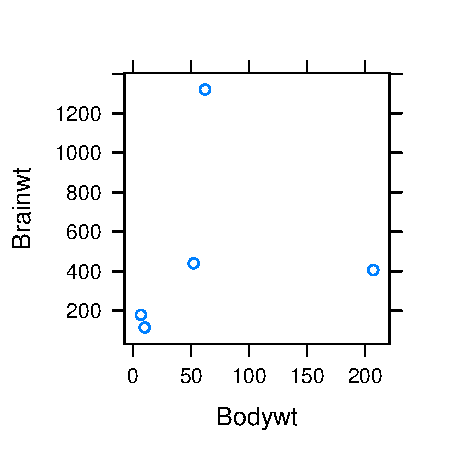
\includegraphics[width=0.97\textwidth]{figs/09-cline-gph-1} }

\end{Schunk}
\caption{Use of lattice function \txtt{xyplot()} to give a graph.
  \label{fig:lat-gph}}
\end{marginfigure}

Figure \ref{fig:lat-gph} was obtained using the lattice function
\txtt{xyplot()}. Superficially, this looks very like the way that
the base graphics function \txtt{plot()} achieves the same end.
Code is:

\begin{Schunk}
\begin{Sinput}
## On the command line: Create and print object
xyplot(Brainwt ~ Bodywt, data=primates)
\end{Sinput}
\end{Schunk}

\subsection*{Lattice graphics functions return graphics objects}
Note an important difference between lattice and base graphics.
Lattice graphics functions do not print graphs.\sidenote{This
  applies also to {\em ggplot2}.} Instead they return
trellis graphics objects.  The graph appears when the object is
printed (use \txtt{print()} or \txtt{plot()}).  Sending the output
from a {\em lattice} graphics function to the command line invokes
\txtt{print()} and the graph is plotted, as was done for Figure
\ref{fig:lat-gph}.

A \txtt{Brainwt} versus \txtt{Bodywt} scatterplot for the
\txtt{primates} data, such as was given earlier, might alternatively
have been obtained using the function the function \txtt{xyplot()}
from the \textit{lattice} package.

\begin{Schunk}
\begin{Sinput}
## Save the result as a trellis graphics object
# [For plot(), this is not possible.]
## Create trellis object
gph <- xyplot(Brainwt ~ Bodywt, data=primates)
## Print graph; a graphics device must now be open
print(gph)
\end{Sinput}
\end{Schunk}
The object \txtt{gph} need not be printed at this point.  It can be
kept for printing at some later time.  Or it can be updated, using the
function \txtt{update()}, and then printed, thus:
\begin{Schunk}
\begin{Sinput}
gph <- xyplot(Brainwt ~ Bodywt, data=primates)
gph2 <- update(gph, xlab="Body wt (kg)",
               ylab="Brain wt (g)")
print(gph2)  # Or it is enough to type 'gph2'
\end{Sinput}
\end{Schunk}

Inside a function\marginnote{The graph will however be
  printed if \txtt{xyplot(...)}  is the final statement
  in a function that returns its result to the command line.}
or in a file that is sourced, \txtt{print()} must
ordinarily be used to give a graph, thus:
\begin{Schunk}
\begin{Sinput}
print(xyplot(ACT ~ year, data=austpop))
\end{Sinput}
\end{Schunk}

\subsection*{Addition of points, lines, text, \ldots}
For adding\sidenote{Do not try to use \margtt{points()} and other
  such base graphics functions with lattice graphs.}
to a plot that has been created using a \textit{lattice} function,
use \verb!panel.points()!, \verb!panel.text()!, and other such
functions, as will be described in Subsection \ref{ss:panel}.

Mechanisms for the control of a wide variety of stylistic
features are best discussed in the context of multi-panel
graphs, which we now consider.

\subsection{Panels of scatterplots}

Graphics functions in the \textit{lattice} package, are designed to
allow row by column layouts of panels.  Different panels are for
different subsets of the data.  Additionally, points can be
distinguished, within panels, according to some further grouping
within the data.

The \txtt{ais} dataset (\textit{DAAG}) has data on elite Australian
athletes who trained at the Australian Institute of Sport. Data were
collected with a view to studying possible differences in blood
characteristics, between athletes in endurance-related events and
those in power-related events.  The help page for \txtt{ais} has
details of the measurements, including a variety of blood cell counts.

A breakdown of the total of 202 athletes by sex and sport gives:
\begin{fullwidth}
\begin{Schunk}
\begin{Sinput}
with(ais, table(sex,sport))
\end{Sinput}
\begin{Soutput}
   sport
sex B_Ball Field Gym Netball Row Swim T_400m T_Sprnt Tennis W_Polo
  f     13     7   4      23  22    9     11       4      7      0
  m     12    12   0       0  15   13     18      11      4     17
\end{Soutput}
\end{Schunk}
\end{fullwidth}
\noindent

Figure \ref{fig:lattice-ais} demonstrates the use of \txtt{xyplot()},
for the rower and swimmer subset os the \txtt{ais} dataset.  The two
panels distinguish the two sports, while different plotting symbols
(on a color device, different colors will be used) distinguish females
from males.
\begin{figure}[h]
\begin{Schunk}


\centerline{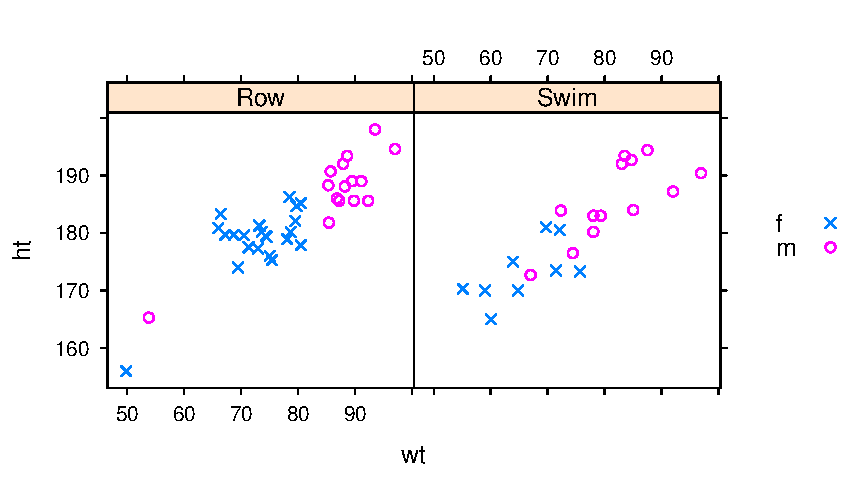
\includegraphics[width=\textwidth]{figs/09-rowSwim-1} }

\end{Schunk}
      \caption{Height (\texttt{ht}) versus Weight (\texttt{wt}), for
        rowers (\texttt{Row}) and swimmers (\texttt{Swim}).
        Different plotting symbols are used to distinguish males from
        females.}\label{fig:lattice-ais}
\end{figure}

\marginnote[11pt]{Use \margtt{auto.key=list(columns=2)} to generate a
  simple key, with items side by side in two columns rather than
  stacked in a single column as is the default
  \margtt{columns=1}.}
\noindent
Suitable code is:
\begin{Schunk}
\begin{Sinput}
xyplot(ht ~ wt | sport, groups=sex, data=ais,
       par.settings=simpleTheme(pch=c(4,1)),
       scales=list(tck=0.5),
       auto.key=list(space="right"),
       subset=sport%in%c("Row","Swim"))
\end{Sinput}
\end{Schunk}
%$

In the graphics formula \verb!ht ~ wt | sport!, the vertical bar
indicates that what follows, in this case \txtt{sport}, is a
conditioning variable or factor.  The graphical information is broken
down by levels of the factor \txtt{sport}.  The parameter
\txtt{aspect} controls the ratio of dimensions in the $y$ and $x$
directions.

The use of the argument \txtt{par.settings}, with its call to
\txtt{simpleTheme} requires explanation, as in the subsection
that now follows.

\subsection{Setting stylistic features}\label{ss:style}

The function \txtt{simpleTheme()} creates a ``theme'', i.e., a list of
settings, that can be supplied via the argument \txtt{par.settings} in
the graphics function call.  Use of the argument \txtt{par.settings}
to a lattice function makes the settings locally, for the specific
graphics object that results.

The \marginnote{Settings that are not available using
  \txtt{simpleTheme()} can if required be added to the theme object
  that \txtt{simpleTheme()} returns. See Subsection
  \ref{ss:latticeParam} has details.}
function \txtt{simpleTheme()} accepts arguments \txtt{col},
\txtt{alpha}, \txtt{cex}, \txtt{pch}, \txtt{lty}, \txtt{lwd},
\txtt{font}, \txtt{fill}, \txtt{border}, plus \txtt{col.points},
\txtt{col.line}, \txtt{alpha.points} and \txtt{alpha.line}.  These
allow separate control (of color and of opacity) for points and lines.

The function \txtt{trellis.device()} opens a new graphics device, with
settings that have in mind the use of {\em lattice} functions. The
function \txtt{trellis.par.set()} sets or changes stylistic features
for the current device. Both these functions accept an argument
\txtt{theme}.\sidenote{Simple variations on the default theme can be
created by a call to \txtt{simpleTheme()}.}  Settings made by
\txtt{trellis.device()} or \txtt{trellis.par.set()} will be
over-written by any local settings that are stored as part of the
graphics object.

\subsection{Groups within data, and/or columns in parallel}\label{ss:grog}

Table \ref{tab:grog} shows selected rows from the data set \txtt{grog}
(\textit{DAAG} package). Each of three liquor products (drinks) has
its own column. Rows are indexed by the factor \txtt{Country}.

% latex table generated in R 2.6.2 by xtable 1.5-2 package
% Mon Mar 31 10:08:43 2008
\begin{table}
\begin{center}
\caption{Apparent annual alcohol consumptiom values, obtained by dividing
    estimates of total available alcohol by number of persons aged 15
    or more. These are based on Australian Bureau of Statistics
    and Statistics New Zealand figures.\label{tab:grog}}
\begin{tabular}{rrrrlr}
  \hline
 & Beer & Wine & Spirit & Country & Year \\
  \hline
1 & 5.24 & 2.86 & 1.81 & Australia & 1998 \\
  2 & 5.15 & 2.87 & 1.77 & Australia & 1999 \\
. . . .\\
  9 & 4.57 & 3.11 & 2.15 & Australia & 2006 \\
  10 & 4.50 & 2.59 & 1.77 & NewZealand & 1998 \\
  11 & 4.28 & 2.65 & 1.64 & NewZealand & 1999 \\
. . . .\\
  18 & 3.96 & 3.09 & 2.20 & NewZealand & 2006 \\
   \hline
\end{tabular}
\end{center}
\end{table}

Figure \ref{fig:allgrog} is one of several possible displays that
might be used to summarize the information in Table \ref{tab:grog}.
It has been created by updating the following simplified code:
\noindent
\begin{Schunk}
\begin{Sinput}
## Simple version of plot
grogplot <- xyplot(
              Beer+Spirit+Wine ~ Year | Country,
              data=grog, outer=FALSE,
              auto.key=list(space="right"))
\end{Sinput}
\end{Schunk}


\begin{figure}
\begin{Schunk}


\centerline{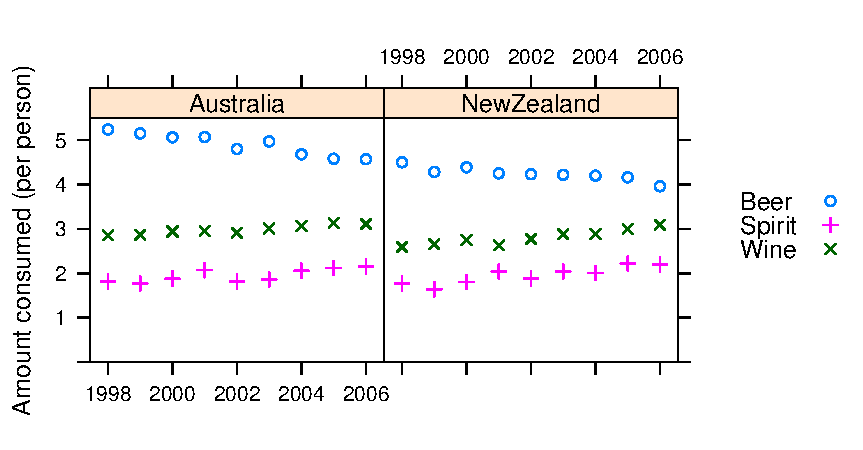
\includegraphics[width=\textwidth]{figs/09-grog-all-1} }

\end{Schunk}
\caption{Australian and New Zealand apparent per person annual
  consumption (in liters) of the pure alcohol content of liquor products, for
  1998 to 2006.  Appendix \ref{app:C} (Figure \ref{col:fig31}) has a color
version of this graph.\label{fig:allgrog}}
\end{figure}

Observe that:
\nopagebreak
\begin{itemizz}
\item[-] Use of \txtt{Beer+Spirit+Wine} gives plots for each of
  \txtt{Beer}, \txtt{Spirit} and \txtt{Wine}.  The effect of
  \margtt{outer=FALSE} is that these appear in the same panel.
\item[-] Conditioning by country (\txtt{$\mid$ Country}) gives separate
  panels for separate countries.
\end{itemizz}

The following updates the object to give Figure \ref{fig:allgrog}:
\marginnote[12pt]{Notice the use of the function \txtt{simpleTheme()}
  to set up a ``theme'' that was used to control point and line
  settings.}
\begin{Schunk}
\begin{Sinput}
## Update trellis object, then print
ylab <- "Amount consumed (per person)"
parset <- simpleTheme(pch=c(1,3,4))
finalplot <- update(grogplot, ylim=c(0,5.5),
                     xlab="", ylab=ylab,
                     par.settings=parset)
print(finalplot)
\end{Sinput}
\end{Schunk}

Figure \ref{fig:allgrog} used different symbols, in the one panel, to
distinguish drinks, with different countries in different panels.
For separate panels for the three liquor products (different levels
of \txtt{Country} can then use the same panel), specify \txtt{outer=TRUE}:
\begin{Schunk}
\begin{Sinput}
xyplot(Beer+Spirit+Wine ~ Year,
       groups=Country, outer=TRUE,
       data=grog, auto.key=list(columns=2) )
\end{Sinput}
\end{Schunk}

Where plots are superposed in the one panel and, e.g., regression
lines or smooth curves are fitted, this is done separately for each
different set of points.  Different colors, and/or by different
symbols and/or line styles, can be used to make the necessary
distinctions.

Here is a summary:
\vspace*{9pt}

\begin{fullwidth}
\begin{tabular}{lccc}
\multicolumn{4}{l}{\bf Break data down a/c to levels of the
factor \texttt{Country}:}\\[3pt]
& Overplot (a single panel): & & Separate panels: \\
& \texttt{Beer $\sim$ Year, groups=Country} & &
\texttt{Beer $\sim$ Year $\mid$ Country}\\[12pt]
\multicolumn{4}{l}{\bf Plot columns in parallel, as in
\texttt{Beer+Wine+Spirit $\sim$ Year}:}\\[3pt]
& Overplot (a single panel): & & Separate panels: \\
& \texttt{outer=FALSE} & & \texttt{outer=TRUE}\\
\end{tabular}
\end{fullwidth}
\pagebreak

\subsection{Keys -- \texttt{auto.key}, \texttt{key} and \texttt{legend}}\label{sec:keys}

The argument \txtt{auto.key=TRUE} gives a basic key.\marginnote{The argument
  \txtt{auto.key} sets up a call \txtt{key=simpleKey()}.  If
  necessary, use \txtt{legend=NULL} when updating, to remove an
  existing key and allow the addition of a new key.} If not otherwise
specified, colors, plotting symbols, and line type use the current
settings for the device.  The argument \txtt{text} has
\txtt{levels(groups)} as its default. that identifies
colors, plotting symbols and names for the groups. For greater
flexibility, \txtt{auto.key} can be a list.  Settings that are often
useful are:
\begin{itemizz}
\item[-] \txtt{points}, \txtt{lines}: in each case set to \txtt{TRUE}
or \txtt{FALSE}.
\item[-] \txtt{columns}: number of columns of keys.
\marginnote[12pt]{\margtt{c(0,0)} is the bottom left corner of the
  legend, etc.}
\item[-] \txtt{x} and \txtt{y}, which are coordinates for
  the whole display area.  Use with \txtt{corner} set
  to one of \txtt{c(0,0)},
  \txtt{c(1,0)}, \txtt{c(1,1)} and \txtt{c(0,1)}.
\item[-] \txtt{space}: one of \txtt{"top"}, \txtt{"bottom"},
\txtt{"left"}, \txtt{"right"}.
\end{itemizz}

\subsection*{$^*$Use of \texttt{textGrob()} to add legends}
The function \txtt{textGrob()} (\textit{grid}) creates a text object
which can then be supplied to the lattice function. This
mechanism for supplying legends can be used when multiple legends are
required.

\begin{marginfigure}[-36pt]
\begin{Schunk}


\centerline{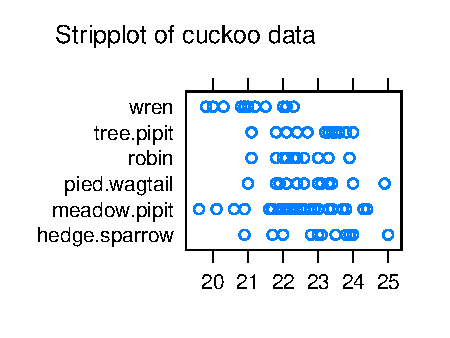
\includegraphics[width=\textwidth]{figs/09-strip-grob-1} }

\end{Schunk}
\caption{The argument \margtt{legend} has been used to add text,
  supplied as a 'grob'.\label{fig:textGrob}. Here, it would be
  easier to use of the argument \margtt{main}.}
\end{marginfigure}

The following code adds an initial legend, as in Figure \ref{fig:textGrob}:
\begin{Schunk}
\begin{Sinput}
plotnam <- "Stripplot of cuckoo data"
stripplot(species ~ length, xlab="", data=cuckoos,
  legend=list(top=list(fun=grid::textGrob,
                       args=list(label=plotnam,
                                 x=0))))
# x=0 is equivalent to x=unit(0,"npc")
# npc units are on a scale from 0 to 1
\end{Sinput}
\end{Schunk}
Additional legends are supplied by adding further
  list elements, for example a list element \txtt{bottom} as well as a
  list element \txtt{top}.

\subsection{Lattice settings -- further notes}\label{ss:latticeParam}

In general, use \txtt{theme}s to make point, line and fill color settings.
Use the \txtt{scales} argument, in the call to the lattice function,
for axes, tick marks, and tick labels.

For changes that go beyond what \txtt{simpleTheme()} allows, first
identify the names under which settings are stored. Type:
\begin{marginfigure}
For a visual display that shows default settings for
  points, lines and fill color, enter:
\begin{Schunk}
\begin{Sinput}
trellis.device(color=FALSE)
show.settings()
trellis.device(color=TRUE)
show.settings()
\end{Sinput}
\end{Schunk}
\end{marginfigure}
\begin{verbatim}
> names(trellis.par.get())
[1] "fontsize"         "background"       "clip"
. . .
[28] "par.sub.text"
\end{verbatim}

The following sets the fontsize, separately for \txtt{text} and
\txtt{points}:\\[-6pt]

\noindent
\begin{minipage}[t]{1.175\textwidth}
\begin{Schunk}
\begin{Sinput}
trellis.par.set(fontsize = list(text = 7,
                                points = 4))
\end{Sinput}
\end{Schunk}
\end{minipage}

\subsection*{Parameters that affect axes, tick marks, and axis labels}
\label{ss:lattice-axis}

These are manipulated by use of the \txtt{scales} argument to
the lattice function. The code for Figure \ref{fig:jobsplot}
provides an example.
\begin{figure*}[h]
\begin{Schunk}


\centerline{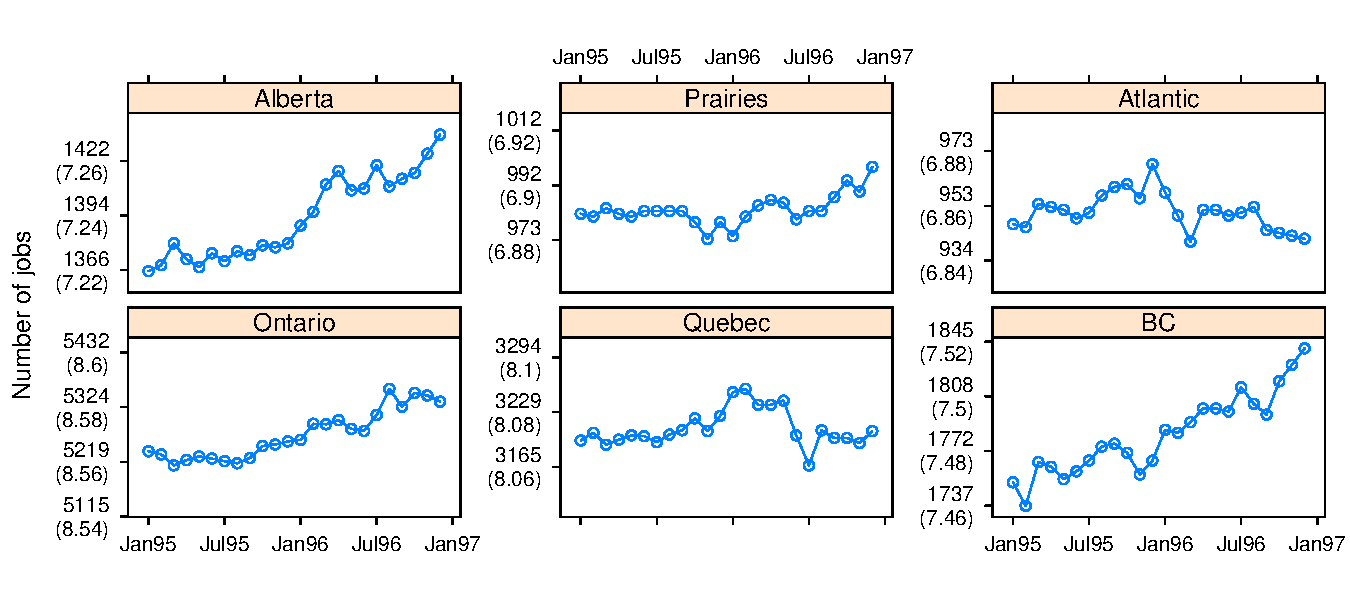
\includegraphics[width=0.97\textwidth]{figs/09-jobsplot-1} }

\end{Schunk}
\caption[][-18pt]{Jobs growth in Canadian provinces, between January 1995
  and December 1996.}\label{fig:jobsplot}
\vspace*{18pt}
\end{figure*}

The following gives a basic graph, which will then be updated:
\noindent
\begin{fullwidth}

\begin{Schunk}
\begin{Sinput}
## 1. Create a basic version of the graphics object
jobsB.xyplot <-
  xyplot(Ontario+Quebec+BC+Alberta+Prairies+Atlantic ~ Date,
         data=jobs, type="b", layout=c(3,2), outer=TRUE,
         ylab="Number of jobs",
         scales=list(y=list(relation="sliced", log=TRUE)))
\end{Sinput}
\end{Schunk}

\end{fullwidth}

\noindent
Now make several enhancements:
\begin{itemizz}
\item[-] Change the $y$-axis labels to show number of jobs, with
$\log(\mbox{number})$ in parentheses underneath.
\item[-] Use dates of the form \txtt{Jan95} to label the
  $x$-axis.\sidenote{Refer back to Subsection \ref{ss:dates}.}
\item[-] Reduce tick marks in length (\txtt{tck=0.6}, i.e.,
60\% of the default).
\item[-] The argument \txtt{between=list(x=0.5, y=0.5)} adds
  horizontal and vertical space between the panels.\sidenote{This
    avoids overlap of tick labels.}
\end{itemizz}

\begin{fullwidth}

\begin{Schunk}
\begin{Sinput}
## 2. Code for the enhancements to jobsB.xyplot
ylabpos <- exp(pretty(log(unlist(jobs[,-7])), 100))
ylabels <- paste0(round(ylabpos),"\n(", log(ylabpos), ")")
## Create a date object 'startofmonth'; use instead of 'Date'
atdates <- seq(from=95, by=0.5, length=5)
datelabs <- format(seq(from=as.Date("1Jan1995", format="%d%b%Y"),
                       by="6 month", length=5), "%b%y")
update(jobsB.xyplot, xlab="", between=list(x=0.5, y=0.5),
       scales=list(x=list(at=atdates, labels=datelabs),
                   y=list(at=ylabpos, labels=ylabels), tck=0.6) )
\end{Sinput}
\end{Schunk}

\end{fullwidth}

\subsection{Lattice plots that show distributions}\label{sec:dists}

\subsection*{Stripplots, dotplots and boxplots}\label{ss:stripetc}

\marginnote[12pt]{Differences between \txtt{dotplot()} and
  \txtt{stripplot()} are mainly cosmetic.}
Because the syntax for \txtt{stripplot()} and \txtt{boxplot()} are
very similar, we demonstrate suitable code side by side.  Figure
\ref{fig:strip-bw} summarizes cuckoo egg length data, from the
dataset \txtt{cuckoos} from \textit{DAAG}:
\vspace*{-9pt}

\begin{figure}
\begin{Schunk}


\centerline{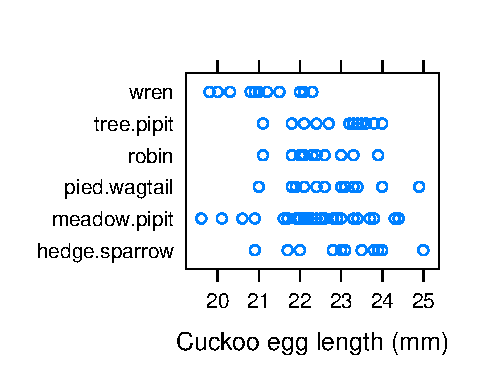
\includegraphics[width=0.47\textwidth]{figs/09-strip-bw-1} 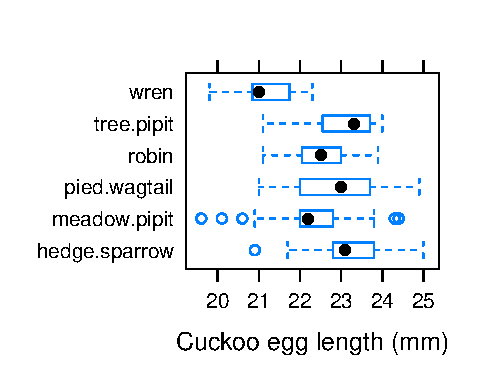
\includegraphics[width=0.47\textwidth]{figs/09-strip-bw-2} }

\end{Schunk}
\caption{A stripplot and a dotplot appear side by side.\label{fig:strip-bw}}
\end{figure}

\begin{Schunk}
\begin{Sinput}
stripplot(species ~ length, data=cuckoos,
          xlab="Cuckoo egg length (mm)")
bwplot(species ~ length, data=cuckoos,
       xlab="Cuckoo egg length (mm)")
\end{Sinput}
\end{Schunk}
\begin{marginfigure}[-36pt]
For slightly improved labeling, precede the code with:
\begin{Schunk}
\begin{Sinput}
levels(cuckoos$species) <-
 sub(".", " ",
  levels(cuckoos$species),
  fixed=TRUE)
\end{Sinput}
\end{Schunk}
\end{marginfigure}
The \txtt{aspect} argument determines the ratio of distance
in the y-direction to distance in the x-direction.

\subsection*{Lattice style density plots}
Here is a density plot (Figure \ref{fig:possumdens}), for data from
the \txtt{possum} data set (\textit{DAAG}), that compares \txtt{sex}es
and \txtt{Vic}/\txtt{other} populations.
\begin{figure}
\begin{center}
\begin{Schunk}


\centerline{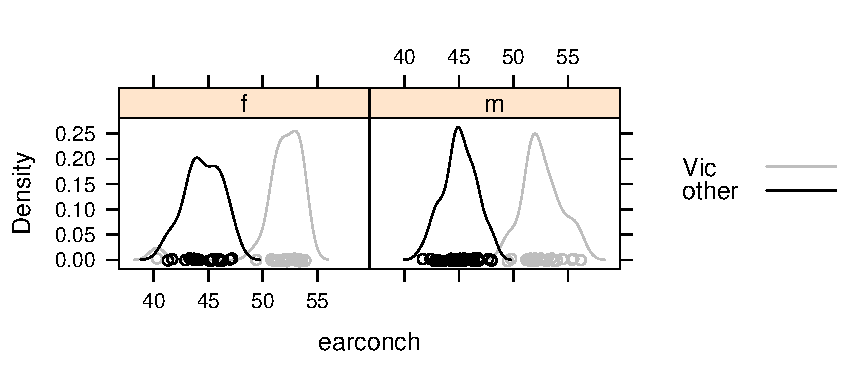
\includegraphics[width=\textwidth]{figs/09-lattice-density-1} }

\end{Schunk}
\end{center}
  \caption{Lattice style density plot comparing possum earconch
    measurements, separately for males and females, between Victorian
    and other populations. Observe that the scatter of data values is
shown along the horizontal axis.}\label{fig:possumdens}
\vspace*{-36pt}
\end{figure}

\begin{Schunk}
\begin{Sinput}
## Code
colset <- c("gray","black")
densityplot(~ earconch | sex, groups=Pop,
            data=possum,
            par.settings=simpleTheme(col=colset),
            auto.key=list(space="right"))
\end{Sinput}
\end{Schunk}
The functions \txtt{densityplot()} and \txtt{histogram()} do not
allow a name on the left of the \txtt{$\sim$} symbol. The function
\txtt{histogram()}, which is otherwise similar to \txtt{densityplot()},
does not accept a \txtt{groups} argument.

\subsection{Panel functions}\label{ss:panel}

\marginnote[11pt]{Subsection \ref{ss:layer} will describe a radical
  extension of this basic scheme. Further layers, created using
  \txtt{layer()} and allied functions in the {\em latticeExtra}
  package can be ``added'' (the operator is ``\txtt{+}'') to a trellis
  graphics object.}  Each lattice function that creates a graphics
object has its own panel function.  Creation of one's own panel
function allows detailed control of panel contents. Or \txtt{update()}
can be used to modify the panel or panels.

A user panel function will typically include, or consist of, calls to
several of the variety of panel functions that are provided in
\textit{lattice}.  The function \txtt{xyplot()} has the panel function
\txtt{panel.xyplot()}.\sidenote{When a \txtt{groups} argument is
  supplied, \texttt{panel.xyplot()} calls the function
  \texttt{panel.superpose()}.}  The following are equivalent:
\begin{Schunk}
\begin{Sinput}
xyplot(species ~ length, xlab="", data=cuckoos)
xyplot(species ~ length, xlab="", data=cuckoos,
       panel=panel.xyplot)
\end{Sinput}
\end{Schunk}
\noindent
A user function, used in place of \txtt{panel.xyplot()},
might for example call \txtt{panel.superpose()},
followed or preceded by other available panel functions.

Available panel functions include:
\begin{itemize}
\item \marginnote[11pt]{Note that an alternative to \texttt{panel.points()}
    is \texttt{lpoints()}. Similarly for the other functions.}
  \txtt{panel.points()},\, \txtt{panel.lines()},\,
  \txtt{panel.text()},\,\\  \verb!panel.rect()!,
  \verb!panel.arrows()!,\, \verb!panel.segments()!, \,\\
  \verb!panel.polygon()!\,\\ (all documented on the same help
  page as \txtt{panel.points()});
\item \txtt{panel.abline()},\, \txtt{panel.curve()},\,
\txtt{panel.rug()}, \,\\  \verb!panel.fill()!,
\txtt{panel.average()},\,\\  \verb!panel.mathdensity()!,\,
 \verb!panel.refline()!,\\
\verb!panel.loess()!, \, \verb!panel.lmline()!\\
(all
documented on the same help page as \txtt{panel.abline()}).
\end{itemize}

The following graphics object \txtt{gph} will be used as a starting
point, in the discussion that now follows:
\begin{Schunk}
\begin{Sinput}
gph <- xyplot(Brainwt ~ Bodywt,  data=primates,
              xlim=c(0,300))
\end{Sinput}
\end{Schunk}

Now create a panel function that both plots the points and adds
labels. The graphics object can then be updated, as in the code that
now follows, to use this panel function:

\begin{marginfigure}[-24pt]
\begin{center}
\begin{Schunk}


\centerline{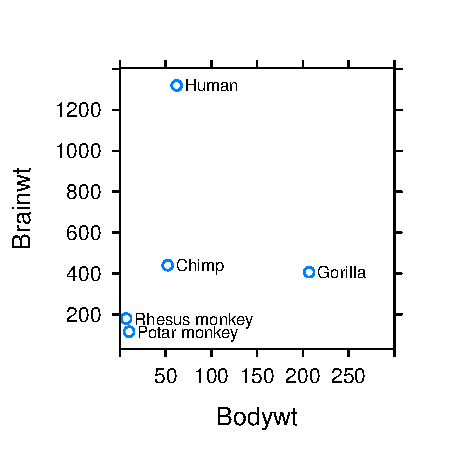
\includegraphics[width=0.98\textwidth]{figs/09-my-panel-1} }

\end{Schunk}
\end{center}
\vspace*{-15pt}

\caption{Addition of labels, as here, can be done by updating a graph
  that has the points, by use of a panel function that both plots
  points and and adds labels, or by adding a new
  layer.}\label{fig:layer}
\end{marginfigure}

\begin{Schunk}
\begin{Sinput}
my.panel <- function(x,y){
  panel.xyplot(x,y)
  panel.text(x,y, labels=rownames(primates),
             cex=0.65, pos=4)
}
update(gph, panel=my.panel,
       scales=list(tck=0.6))
\end{Sinput}
\end{Schunk}

Note that we could have supplied a panel function that plots
the points and adds the labels in the initial function call, thus:
\begin{Schunk}
\begin{Sinput}
xyplot(Brainwt ~ Bodywt, data=primates,
       xlim=c(0,300), panel=my.panel)
\end{Sinput}
\end{Schunk}

A further possibility is to add a new layer that has the labels, as
in Subsection \ref{ss:layer} which now follows.
However the plot is obtained, Figure \ref{fig:layer} shows the result.

\subsection{The addition of new layers}\label{ss:layer}
The layering mechanism greatly extends the range of possibilities.
The code that follows gives a simple and somewhat trivial example
of its use -- an alternative the use of a panel function for adding
labeling to Figure \ref{fig:layer}.

Note again the graphics object \txtt{gph}, created above:
\begin{Schunk}
\begin{Sinput}
gph <- xyplot(Brainwt ~ Bodywt,  data=primates,
              xlim=c(0,300))
\end{Sinput}
\end{Schunk}
\noindent
The following uses the function \txtt{layer()}, from the
\textit{latticeExtra} package, to create a second layer that has the
labels. The layer that is thus created is added to the graphics object
\txtt{gph}:
\begin{Schunk}
\begin{Sinput}
gph + latticeExtra::layer(panel.text(x,y,
                       labels=rownames(primates),
                       pos=4))
\end{Sinput}
\end{Schunk}
\noindent Note also
\texttt{layer\_()}, which reverses the order of the layers,
equivalent to using \txtt{layer()} with \txtt{under=TRUE}.
\marginnote[-12pt]{Other convenience functions are \texttt{glayer()} and
  \texttt{glayer\_()}.  These are equivalent, respectively, to calling
  \texttt{layer()} and \texttt{layer\_()} with
  \texttt{superpose=TRUE}. The layer is drawn once for each level of
  any group in the plot.}

The function \txtt{layer()} allows as arguments,
passed via the \txtt{\ldots} argument, any sequence of statements
that might appear in a panel function.  Such statements can refer to
panel function arguments, including 'x', 'y' and 'subscripts'.
Additionally, named column objects can be passed through an optional
\txtt{data} argument.

The function \txtt{as.layer()} creates a layer from a trellis graphics
object.  This can then be ``added'' in the usual way.

\subsection{Interaction with plots -- \textit{latticist} and
  \textit{playwith}}\label{ssec:playwith}

\marginnote[-24pt]{For using \textit{playwith}, the GTK+ toolkit must
  be installed. For details, go to the website {\scriptsize
    \url{http://playwith.googlecode.com/}.}}  Here will be noted the
abilities in the \textit{latticist} and \textit{playwith} packages,
for interaction with lattice plots.\sidenote{More limited abilities
  are available to interact with other plots.}

\paragraph{\texttt{latticist()}:}
When called with a data frame as argument, the function
\txtt{latticist()} (in the \textit{latticist} package) opens a
window that has graphical summary information on the columns of the
data frame.  Additionally, it opens a GUI interface to the
\textit{lattice} and \textit{vcd} packages, allowing rapid creation of
plots that may be useful in their own right, or may be a first step in
creating more carefully crafted plots.  Various annotation features
are available from the GUI.

\paragraph{\texttt{playwith()}:}
The \texttt{playwith()}  function (from the \textit{playwith}
package) was used for Figure \ref{fig:playwith}.  The menu that
appears to the left of the graph can be used to initiate single
click identification, to add annotation or arrows, or to mark
out a rectangle on the graph for zooming in or out.  If labels
are not specified, row names are used.
\vspace*{6pt}

\begin{figure}[h]
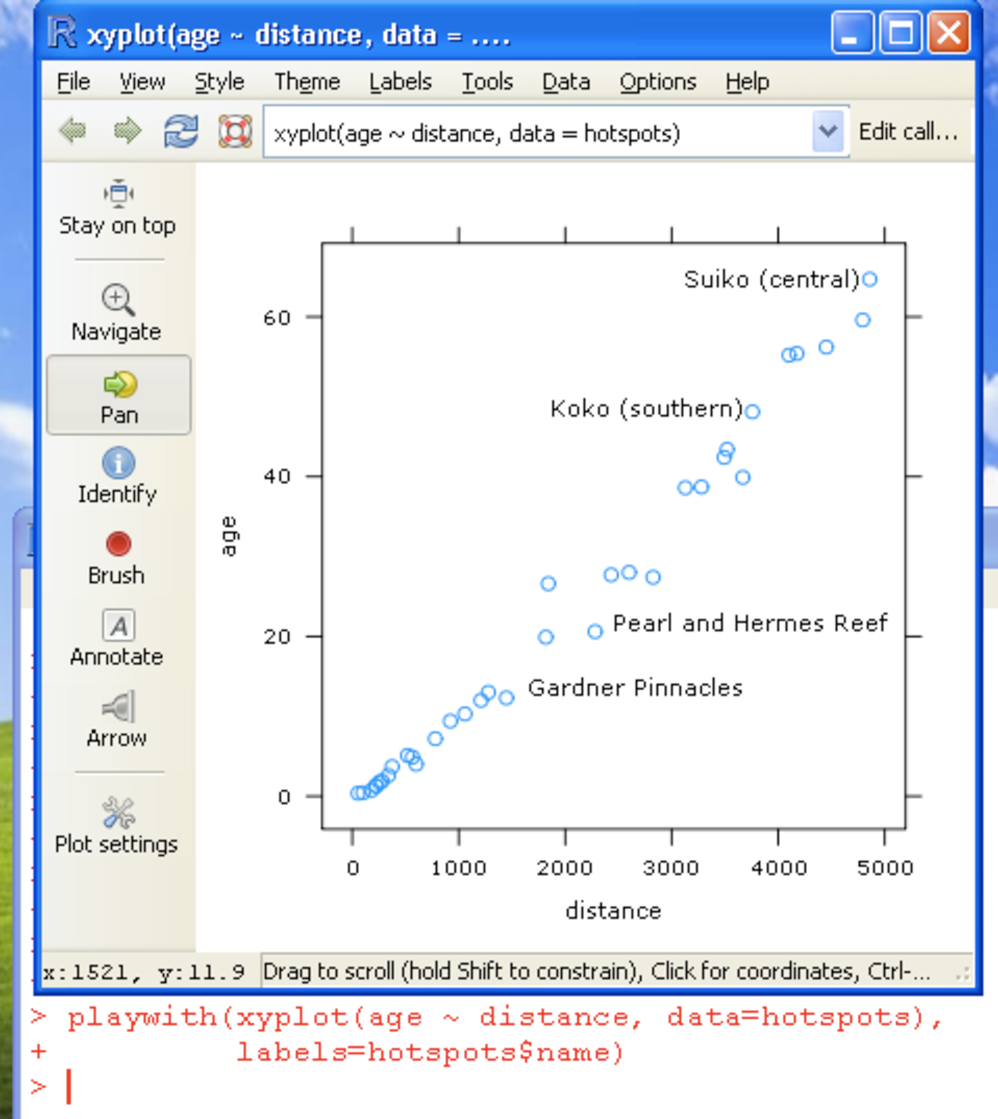
\includegraphics[scale=0.65]{colorArt/playwith}%
\caption{This playwith GUI window was generated by wrapping the call
  to \texttt{xyplot()} in the function \texttt{playwith()}, then
  clicking on \underline{Identify}. Click near to a point to see its
  label. A second click adds the label to the graph.  A color version
appears as \ref{col:playwith}.\label{fig:playwith}}
\end{figure}
\vspace*{6pt}

\begin{Schunk}
\begin{Sinput}
## Code that initiates interactive display
library(playwith)
playwith(xyplot(age ~ distance, data=hotspots),
         labels=hotspots$name)
\end{Sinput}
\end{Schunk}
\begin{marginfigure}[-24pt]
Alternative code for Figure \ref{fig:playwith}:\\[-3pt]
\begin{Schunk}
\begin{Sinput}
gph <-
    xyplot(age ~ distance,
            data=hotspots)
library(playwith)
playwith(update(gph),
    labels=hotspots$name)
\end{Sinput}
\end{Schunk}
\end{marginfigure}

Note that \txtt{playwith()} can be used, also, for more limited
interaction with plots created using base graphics, or
using \textit{ggplot2}.


\section{\textit{ggplot2} -- A \textit{Grammar of  Graphics}}\label{sec:ggplot}

\marginnote{The \textit{ggplot2} syntax is a variant of
  Wilkinson's ``Grammar of Graphics''
  (Springer, 2$^{nd}$ edn, 2005).}

The {\em ggplot2} syntax is consistent, but less stylized than the
\textit{lattice} syntax.  As with \textit{lattice}, {\em ggplot2}
functions return a graphics object. The graphics objects that {\em
    ggplot2} functions return can be saved for later use, or updated,
  or printed directly on to the graphics page. Each different type of
{\em ggplot2} graphic display -- scatterplot, histogram, density plot,
histogram, etc. -- is a different plot \txtt{geom}, or
``geometry''.  These can be overlaid.

The following loads the {\em ggplot2} package:
\begin{Schunk}
\begin{Sinput}
library(ggplot2)
\end{Sinput}
\end{Schunk}

\subsection{Examples that demonstrate ggplot2 abilities}

\subsection*{Brain weight versus body weight}
Figure \ref{fig:ggplot2-brain} repeats Figure \ref{fig:Animals}B from Chapter
\ref{ch:worked}, now using {\em ggplot2} abilities:
\begin{figure}
\begin{Schunk}


\centerline{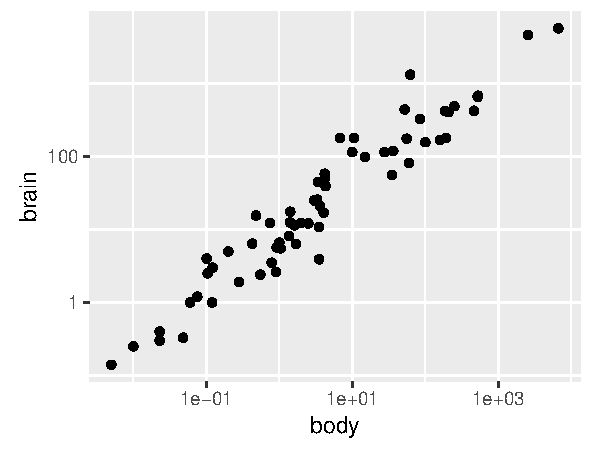
\includegraphics[width=0.7\linewidth]{figs/09-ggplot2-brain-1} }

\end{Schunk}
\caption{Plot of brain weight (gm) versus body weight (kg).
Log scales have been used on both axes.  The function
\txtt{coord\_equal()}, used with a logarithmic scale, ensures
that a given distance (e.g., 1cm) on either axis represents
the same relative change.\label{fig:ggplot2-brain}}
\end{figure}

\noindent Code is:
\begin{Schunk}
\begin{Sinput}
library(MASS)
quickplot(body, brain, data=mammals, log="xy") +
  coord_fixed()
\end{Sinput}
\end{Schunk}
\marginnote[12pt]{In subsequent discussion, the abbreviated name
  \margtt{qplot} will be used in place of \margtt{quickplot}.}  Notice
that \txtt{quickplot()} has been used to create an initial plot, with
\txtt{coord\_equal()} then used (``added'') to specify that a given
distance will represent the same change on both axes.  As a
logarithmic scale is used, this implies that the same relative change
will be given by the same distance.  Here, observe that grid lines in
both directions are the same distance apart, with the distance
representing a change by a factor of 100,

The following adds a regression line:
\begin{Schunk}
\begin{Sinput}
quickplot(body, brain, data=mammals, log="xy") +
  coord_fixed() +
  geom_smooth(method=lm)
\end{Sinput}
\end{Schunk}
This ``addition'' of new functions that add to or modify the
initial graph can in principle proceed without limit.

As the name hints, the function \txtt{qplot()} (or \txtt{quickplot()})
shortcuts the more detailed {\em ggplot2} syntax.  The call
\begin{Schunk}
\begin{Sinput}
quickplot((body, brain, data=mammals, log="xy")
\end{Sinput}
\end{Schunk}
when written out using the detailed syntactic steps, becomes:
\begin{Schunk}
\begin{Sinput}
ggplot(mammals, aes(body, brain)) +
  geom_point() +
  scale_x_continuous(trans="log") +
  scale_y_continuous(trans="log")
\end{Sinput}
\end{Schunk}
The successive ``\txtt{+}'' operators combine output from
function calls to create a single graphics object.  In the
detailed syntactic steps, the call to \txtt{geom\_point()}
plots the points, while the subsequent calls change the
$x$- and $y$-axis scales to logarithmic scales.

In the call to \txtt{ggplot()}, the \txtt{data} argument is the
only mandatory argument. It can be repeated in the call(s) to one
or more of the later \txtt{geom} functions. This allows different
\txtt{geom}s, if required, to take their data from different data
frames.

\marginnote[12pt]{Note that \margtt{cex} and \margtt{size}
are synonyms, as are \margtt{color} and \margtt{colour}.  Also
\margtt{type} is a synonym for \margtt{geom}.}
Changes to \txtt{color} or \txtt{size} or \txtt{shape} settings
can be made separately for each different \txtt{geom}.
Changing \verb!geom_point()!  to \verb!geom_point(size=2.5)! affects
only the points.

\subsection*{Aesthetic mappings vs settings}\label{ss:I(size)}

Distinguish between {\em settings} and {\em aesthetic mappings}:\\[4pt]
\hspace*{6pt}
\begin{fullwidth}
\begin{tabular}{llll}
&  Use of \texttt{quickplot()} && Plots based on \texttt{ggplot()}\\
\cline{2-2} \cline{4-4}
Settings &  \texttt{size=I(3)} or \texttt{cex=3}&&
\texttt{size=3}\\
Aesthetic mappings & \texttt{size=3} or \texttt{size=sport} &&
\texttt{aes(size=3)} or \texttt{aes(size=sport)}\\
\cline{2-2} \cline{4-4}
\end{tabular}\\[8pt]
\end{fullwidth}
The function \txtt{aes()} maps variables in the data to visual
properties (``aesthetics'') of \txtt{geom}s.  In \txtt{aes(body,
  brain} above, the mappings are to the $x-$ and $y-$axes of the plot.
Other possible mappings are to \txtt{color} (use color to distinguish
groups within the data), \txtt{shape}\sidenote{Where base graphics has
  \txtt{pch}, {\em ggplot2} has \txtt{shape}.}  (distinguish by
shape), \txtt{size} and \txtt{fill}.

Use of the argument \txtt{size=3} in a call to \txtt{quickplot()}
does change the point size, but it adds an extraneous key.
The same happens if the argument \txtt{mapping=aes(size=3)}
is supplied to \txtt{ggplot()} or to \txtt{geom\_point()} or
to another such function.

A further possibility is to use \txtt{quickplot()} (or \txtt{qplot()})
to create an initial graphics object, then adding to this object. The
following code uses this approach to create Figure \ref{fig:ggrain}:
\begin{Schunk}
\begin{Sinput}
qplot(Year, mdbRain, data=bomregions2015,
      geom="point",
      xlab="", ylab="Av. rainfall, M-D basin") +
  geom_smooth(span=0.5, se=TRUE)
\end{Sinput}
\end{Schunk}

In all cases, a \txtt{ggplot} object is created. This can
be \txtt{print}ed immediately, or it can be saved as a named object.
The graph is created using the \txtt{print} method for a
\txtt{ggplot} object.

\subsection{An overview of {\em ggplot2} technicalities}




\subsection*{Available geometries and settings}

Table \ref{tab:geom} has details of a number of the geometries that
are available for \txtt{ggplot} objects. Table \ref{tab:cmpts} lists
some of the settings, in addition to those already noted, that are
available:\\[-9pt]
\begin{fullwidth}
\begin{table}
\caption{Available \texttt{geom}s.\label{tab:geom}}
\begin{center}
\vspace*{18pt}

\begin{minipage}[t]{0.975\textwidth}
\setcounter{mpfootnote}{\value{footnote}}
\renewcommand{\thempfootnote}{\arabic{mpfootnote}}
\hspace*{6pt} \begin{tabular}{lllll}
  \texttt{quickplot()} && \texttt{ggplot()} && Available arguments to
  the \texttt{geom} function\\
\cline{1-1} \cline{3-3} \cline{5-5}
\texttt{geom=} &&  && (\texttt{data}, \texttt{mapping},
\texttt{color}, \texttt{fill}, \texttt{alpha}, plus \ldots)\\
\cline{1-1} \cline{3-3} \cline{5-5}
  \texttt{"point"} &&\verb!+ geom_point()! && \texttt{size},
  \texttt{shape}, etc.\\
  \texttt{"line"} &&\verb!+ geom_line()! &&
  \texttt{size}, \texttt{linetype}
  \\
  \texttt{"path"} &&\verb!+ geom_path()!\footnotemark[1] &&
  \texttt{size}, \texttt{linetype}
  \\
  \texttt{"smooth"} &&\verb!+ geom_smooth()! &&
  \texttt{linetype},
  \texttt{weight}, \texttt{se} (\texttt{TRUE} or \texttt{FALSE}).
  \\
  \texttt{"histogram"} &&\verb!+ geom_histogram()! &&
  \texttt{linetype}, \texttt{weight}
  \\
  \texttt{"density"} &&\verb!+ geom_density()! &&
\texttt{weight},  \texttt{linetype}, \texttt{size}
\\
  \texttt{"density2d"} &&\verb!+ geom_density2d()! &&
\texttt{weight},  \texttt{linetype}, \texttt{size}\\
\end{tabular}
\footnotetext[1]{Use \texttt{geom\_path()} to connect
  observations, in the original order.}
\setcounter{footnote}{\value{mpfootnote}}
\end{minipage}
\end{center}
\end{table}
\end{fullwidth}

\begin{fullwidth}
\begin{table}%
\caption{Control of ggplot2 graphics features. Note that functions
  such as \txtt{xlab()} and \txtt{scale\_x\_continuous()} all have
  counterparts with \txtt{y} in place of \txtt{x}.
  \label{tab:cmpts}.}
\vspace*{60pt}

\begin{center}
\begin{minipage}[t]{0.975\textwidth}
\setcounter{mpfootnote}{\value{footnote}}
\renewcommand{\thempfootnote}{\arabic{mpfootnote}}
\begin{tabular}{@{}l@{\hskip 9pt}ll@{\hskip 4pt}l}%
  & Argument to \texttt{qplot()} && \texttt{ggplot()} or
  \txtt{qplot()}\footnotemark[1]\\
\cline{2-2} \cline{4-4}
Title & \texttt{main="mytitle"} && \texttt{+ labs(title="mytitle")}\\
 Axes & see \txtt{help(qplot)} &&
\txtt{+ scale\_x\_continuous()}\footnotemark[2] \\
 &&& \quad[or \txtt{scale\_x\_discrete()} or \txtt{scale\_x\_date()}] \\
  Axis labels & e.g., \texttt{xlab="myxlab"} &&
  \texttt{+ xlab("myxlab")}\footnotemark[3]\\
log axes & \txtt{log="x"}, (or \txtt{"y"}, or \txtt{"xy"}) &&
\txtt{+ scale\_x\_log10()}\footnotemark[4] \\
  Facets\footnotemark[5] & \txtt{facets=sex \textasciitilde\ sport} &&
  \txtt{+ facet\_grid(sex \textasciitilde\ sport)} \\
Aspect ratio & e.g., \txtt{asp=1} &&
\texttt{+ coord\_equal()}\footnotemark[6]\\
Theme & --- && \\
Graph title & e.g., \texttt{main="maintitle"} &&
  \txtt{+ ggtitle("mytitle")}\\
% \cline{2-2} \cline{4-4}
\end{tabular}
\footnotetext[1]{Recall that \texttt{quickplot()} (or
  \txtt{qplot()}) returns a \texttt{ggplot} object. Functions such as
  \txtt{xlab()} or \txtt{scale\_x\_continuous()} can be used, just as
  for any other ggplot2 object, to update objects returned by
  \txtt{quickplot()}.}
\footnotetext[2]{Available arguments include
  \txtt{limits}, \txtt{breaks} (locations for the ticks),
  \txtt{labels} (labels for the breaks), and \txtt{trans} (e.g.,
  \txtt{trans="log"}).}
\footnotetext[3]{This is an alternative to using \txtt{name}
  (e.g., \texttt{name="myxlab"}) as an argument to
  \texttt{scale\_x\_continuous()} or
  \texttt{scale\_x\_discrete()}.}
\footnotetext[4]{This is an alternative to using
  \txtt{trans="log10"} as an argument to \texttt{scale\_x\_continuous()}
  or \texttt{scale\_x\_discrete()}.  Note also \txtt{trans="log"} and
  \txtt{trans="log2"}).}
\footnotetext[5]{Facets give Lattice style {\em conditioning}.}
\footnotetext[6]{By default (\texttt{ratio=1}), a given distance, e.g.,
  1cm, represents the same range along both $x-$ and $y-$axes.}
\footnotetext[7]{Themes control such graphical attributes as background color, gridlines,
and size and color of fonts.  See \txtt{help(ggtheme)} for details of other available
themes.}
\setcounter{footnote}{\value{mpfootnote}}
\end{minipage}
\end{center}
\end{table}
\end{fullwidth}
\enlargethispage{9pt}

\subsection*{Example --- Measurements on Australian athletes}

Figure \ref{fig:ggais} plots height against weight, by sex, for the
\txtt{ais} data. Additionally, boxplots show the distributions of
heights, and there are two-dimensional density contours estimates.
The graph is a tad crowded.

\begin{figure}
\begin{Schunk}


\centerline{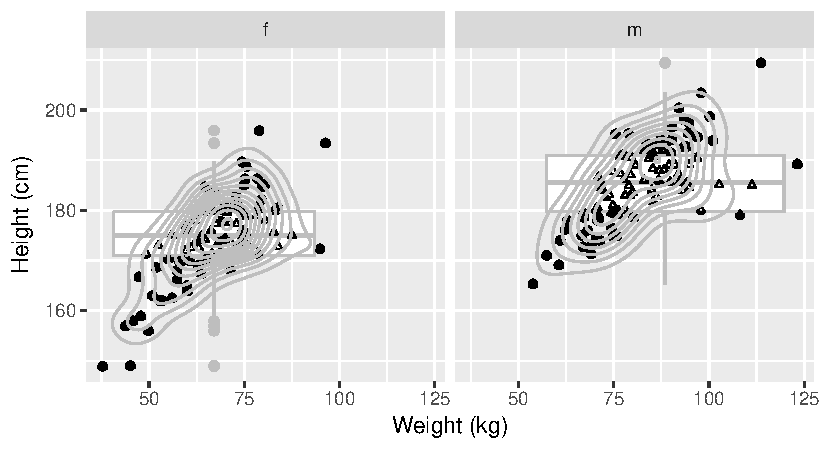
\includegraphics[width=\textwidth]{figs/09-overlay-dens-frills-1} }

\end{Schunk}
\caption{Height versus weight, by sex, for Australian athletes in the
\texttt{ais} data set. Boxplots that show the distributions of heights,
and two-dimensional density contours have been
added.\label{fig:ggais}}
\end{figure}

The following gives a simplified version of the plot:\vspace*{-3pt}
\begin{Schunk}
\begin{Sinput}
## Overlay with boxplots and density contours
quickplot(wt, ht, data=ais,
          geom=c("boxplot", "point", "density2d"),
          facets = . ~ sex)
\end{Sinput}
\end{Schunk}
To set axis labels, show the boxplot outline in gray, show contour
lines in gray (the default is blue), and make various other changes
as in Figure \ref{fig:ggais}, specify:\vspace*{-3pt}
\begin{Schunk}
\begin{Sinput}
quickplot(wt, ht, xlab="Weight (kg)",
          ylab="Height (cm)", data=ais,
          facets = . ~ sex) +
  geom_boxplot(aes(group=sex),
               outlier.size=1.75,
               outlier.colour="gray",
               color="gray") +
  geom_point(shape=2, size=1) +
  geom_density2d(color="gray")
\end{Sinput}
\end{Schunk}

The \txtt{facets} argument has the form \verb!row.var ~ col.var!,
where \txtt{row.var} indexes rows of panels, \txtt{col.var}
indexes columns, and ``\txtt{.}'' serves as a placeholder when there is
one row or one column only.

Code for the next plot will work with a subset of the \txtt{ais}
data, limiting attention to rowers and swimmers:
\begin{Schunk}
\begin{Sinput}
## Extract from ais data for rowers and swimmers
aisRS <- subset(ais, sport %in% c("Row","Swim"))
aisRS$sport <- droplevels(aisRS$sport)
\end{Sinput}
\end{Schunk}

\begin{marginfigure}[-72pt]
\begin{Schunk}


\centerline{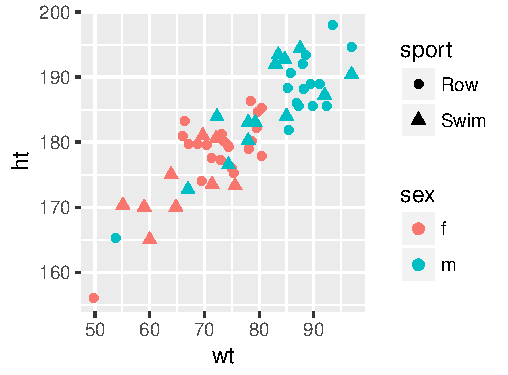
\includegraphics[width=\textwidth]{figs/09-quick-rs1-1} }

\end{Schunk}
\caption{Use \texttt{color} for distinguishing \texttt{sex}es,
\texttt{shape}s for \texttt{sport}s.
Figure \ref{col:colshape} in Appendix \ref{app:C}
shows the graph in color.}\label{fig:colshape}

\end{marginfigure}

Here are alternative code fragments that can be used to create
Figure \ref{fig:colshape}, one using \txtt{quickplot()} and the other
using successive calls to \txtt{ggplot()} and to \txtt{geom\_point()}:
\vspace*{9pt}

\begin{fullwidth}
\begin{minipage}[t]{0.36\linewidth}
{\bf 1: Use \txtt{quickplot()}:}
\begin{Schunk}
\begin{Sinput}
quickplot(wt, ht,
          data=aisRS,
          geom="point",
          size=I(2),
          colour=sex,
          shape=sport)
\end{Sinput}
\end{Schunk}
\end{minipage}
\hspace*{0.04\textwidth}
\begin{minipage}[t]{0.4\linewidth}
{\bf 2: \txtt{ggplot() + geom\_point()}:}
\begin{Schunk}
\begin{Sinput}
ggplot(aisRS) +
  geom_point(aes(wt, ht,
               color=sex,
               shape=sport),
             size=2)
\end{Sinput}
\end{Schunk}
\end{minipage}
\end{fullwidth}

Multiple aesthetics can be used for the one distinction, here
between \txtt{sex}es:
\begin{Schunk}
\begin{Sinput}
## Distinguish sex by color & shape
## Different sports have different panels
quickplot(wt, ht, data=aisRS, geom="point",
          size=I(2.5), color=sex, shape=sex,
          facets = . ~ sport)
\end{Sinput}
\end{Schunk}

Here are further possibilities:
\begin{Schunk}
\begin{Sinput}
## Identify sex by color, sport by shape (1 panel)
quickplot(wt, ht, data=aisRS, geom="point",
           color=sex, shape=sport, size=I(2.5))
## Identify sex by color, sport by size (1 panel)
quickplot(wt, ht, data=aisRS, geom="point",
          color=sex, size=sport)
\end{Sinput}
\end{Schunk}

\subsection*{Australian rain data}

 Figure \ref{fig:ggrain} plots annual rainfall for Australia's
 Murray-Darling basin region. The following code uses the
 function \txtt{quickplot()}:

\begin{Schunk}
\begin{Sinput}
library(DAAG)
library(ggplot2)
## Default loess smooth, with SE bands added.
quickplot(Year, mdbRain, data=bomregions2015,
          geom=c("point","smooth"), xlab="",
          ylab="Av. rainfall, M-D basin")
\end{Sinput}
\end{Schunk}
\marginnote[-60pt]{Arguments \txtt{size} (e.g., \txtt{size=I(2.5)}),
  \txtt{color} (e.g., \txtt{color=I("red")}, etc, can be supplied,
  affecting both points and the added smooth curve. NB:
  \txtt{size=I(2.5)}, not \txtt{size=2.5}.}

\begin{figure}
\begin{Schunk}


\centerline{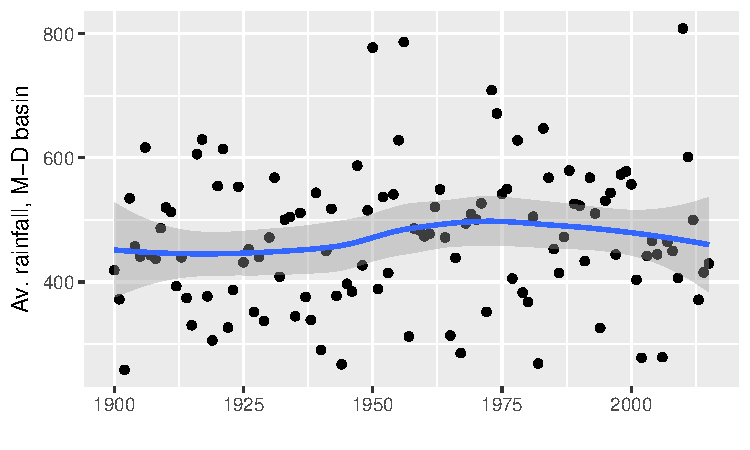
\includegraphics[width=\textwidth]{figs/09-qplot-smooth-1} }

\end{Schunk}
\caption{Annual rainfall, from 1901 to 2012, for the Murray-Darling
  basin region of Australia.  The curve is fitted using the default
  loess smoother. The pointwise standard error bands assume that
  errors about the curve are independent; this is unlikely to be
  strictly true. To suppress these bands, specify
  \texttt{se=FALSE}.\label{fig:ggrain}}
\end{figure}

Code that shows the detailed syntactic steps is:

As before, the successive ``\txtt{+}'' operators combine output from
function calls to create a single graphics object.

Try also the following.  This requires both the {\em quantreg}
package and the {\em splines} package:
\marginnote[12pt]{The normal spline basis \txtt{ns(x,5)} is supplied to the
function that estimates the quantile curves, so that 5 d.f.\ spline
curves are fitted at the 20\%, 50\% and 80\% quantiles.}
\begin{Schunk}
\begin{Sinput}
library(quantreg)
library(splines)
## Supplementary figure 4
quickplot(Year, mdbRain, data=bomregions2015) +
          geom_quantile(formula = y ~ ns(x,5),
          quantiles=c(0.2,0.5,0.8) )
\end{Sinput}
\end{Schunk}

\subsection*{Florence Nightingale's Wedge Plot}
\marginnote[-0.5cm]{Florence Nightingale's Crimean War experience
  prepared her for later major work in the reform of army and
  civilian hospitals and public health administration, and to wider
  social reform.  Her influence extended to the army and civilian
  administration in India.}

Figure \ref{col:wedgeplot} in Appendix \ref{app:C} is a ``wedge''
plot, showing the mortality of British troops according to cause in
the Crimean war over 1854--1856. It shows the abilities of the {\em
  ggplot2} package to spectacular effect.  The plot is obtained by
using polar coordinates for plotting a stacked bar chart!  Use of
areas to convey numerical information is however not ideal, especially
when as here the areas overlap.


\section{Graphics -- Additional Points}
\subsection{Multiple graphs on a single graphics page}\label{ssec:xgph}

For \textit{base} graphics, refer back to Subsection \ref{ss:xplots}.
The following demonstrates use of the \txtt{fig}
argument to \txtt{par()} to select a part of the display region
for plotting:
\begin{Schunk}
\begin{Sinput}
par(fig = c(0, 1, 0.38, 1))
          # xleft, xright, ylow, yhigh
## Plot graph A
par(fig = c(0, 1, 0, 0.38), new=TRUE)
## Plot graph B
par(fig = c(0, 1, 0, 1))     # Resets to default
\end{Sinput}
\end{Schunk}
For lattice graphs, the location of the graph can be determined
by the argument \txtt{position}, when \txtt{print()} is called.
The following demonstrates its use:
\begin{fullwidth}
\begin{Schunk}
\begin{Sinput}
cuckoos.strip <- stripplot(species ~ length, xlab="", data=cuckoos)
print(cuckoos.strip, position=c(0,0.5,1,1))
                   # xleft, ybottom, xright, ytop
cuckoos.bw <- bwplot(species ~ length, xlab="", data=cuckoos)
print(cuckoos.bw, position=c(0,0,1,0.5), newpage=FALSE)
\end{Sinput}
\end{Schunk}
\end{fullwidth}
\noindent
Note the use of \txtt{newpage=FALSE} for the second plot.

\subsection*{Base and trellis plots on the same graphics page}

The following uses the base graphics command \txtt{mtext()}
to label a lattice plot:
\begin{Schunk}
\begin{Sinput}
plot(0:1, 0:1, type="n", bty="n", axes=FALSE,
     xlab="", ylab="")
lab <- "Lattice bwplot (i.e., boxplot)"
mtext(side=3, line=3, lab)
cuckoos.bw <- bwplot(species~length, data=cuckoos)
print(cuckoos.bw, newpage=FALSE)
\end{Sinput}
\end{Schunk}

\subsection*{Inclusion of graphs in Microsoft Word}

Graphs may not import well from the clipboard into Word on the
Macintosh under OS X.  On Windows systems, an effective option is to
use \txtt{win.metafile()} to write graphics output to a Windows
metafile format that should import without problem into a Word or
Power Point document.

\section{Summary}
\begin{itemize}
\item[] Base graphics functions plot a graph.  Lattice and ggplot2
functions return a graphics object. which can then stored or updated
or plotted (printed).

\item[] A powerful feature, both of \textit{ggplot2} graphics and of
  \textit{lattice} graphics when the layering abilities of the
  \textit{latticeExtra} package is used, is the ability to build a
  graph up layer by layer.

\item[] The R system makes available, via its various package,
a wide variety of other graphics abilities.  This includes
dynamic and other 3-dimensional graphics.
\end{itemize}


\section{Exercises}\label{sec:plot}
In the following exercises, if there is no indication of whether to
use \txtt{base} or \txtt{lattice} graphics, use whichever seems
most suitable.

\begin{enumerate}
\item Exercise \ref{ex:mol1} in Section \ref{ss:wd} showed how to
create the data frame \txtt{molclock}.  Plot \txtt{AvRate}
  against \txtt{Myr}. Use \txtt{abbreviate()} to create abbreviated
  versions of the row names, and use these to label the
  points.\label{ex:molclock}

\item Compare the following graphs that show the distribution of head
  lengths (\txtt{hdlngth}) in the \txtt{possum} data set.
What are the advantages and disadvantages of these different
forms of display?
\begin{itemizz}
\item[] a) a histogram (\txtt{hist(possum\$hdlngth))};

\item[] b) a stem and leaf plot (\txtt{stem(qqnorm(possum\$hdlngth))};

\item[] c) a normal probability plot (\txtt{qqnorm(possum\$hdlngth))};
and

\item[] d) a density plot (\txtt{plot(density(possum\$hdlngth)).}
\end{itemizz}

\item This exercise uses the data set \txtt{hotspots}
  (\textit{DAAG} package).

Plot \txtt{age} against \txtt{distance}.  Use \txtt{identify()} to
determine which years correspond to the two highest mean levels. That
is, type
\begin{Schunk}
\begin{Sinput}
plot(age ~ distance, data=hotspots)
with(hotspots, identify(age ~ distance, labels=name))
\end{Sinput}
\end{Schunk}
% $
Use the left mouse button to click on the highest two points
on the plot. (Right click in the figure region to terminate labeling.)

\item Use \txtt{mfrow()} to set up the layout for a 3 by 4 array
of plots. In the top 4 rows, show normal probability plots
for four separate `random' samples of size 10, all from
a normal distribution. In the middle 4 rows, display plots for
samples of size 100. In the bottom four rows, display plots for
samples of size 1000. Comment on how the appearance of the plots
changes as the sample size changes.

\item The function \txtt{runif()} can be used to generate a sample
  from a uniform distribution, by default on the interval 0 to
  1. Print out the numbers you get from \txtt{x \txtt{<}-
    runif(10)}. Then repeat exercise 6 above, but taking samples from
  a uniform distribution rather than from a normal distribution.  What
  shape do the points follow?

\item The data frame \txtt{airquality} that is in the base package has
  columns \txtt{Ozone}, \txtt{Solar.R}, \txtt{Wind},
  \txtt{Temp}, \txtt{Month} and \txtt{Day}. Plot
  \txtt{Ozone} against \txtt{Solar.R} for each of three
  temperature ranges, and each of three wind ranges.
\item Create a version of the data frame \texttt{Pima.tr2} that has
  \texttt{anymiss} as an additional column:
\begin{Schunk}
\begin{Sinput}
missIND <- complete.cases(Pima.tr2)
Pima.tr2$anymiss <- c("miss","nomiss")[missIND+1]
\end{Sinput}
\end{Schunk}
\begin{itemize}
\item[(a)] Use strip plots to compare values of the various measures for
the levels of \texttt{anymiss}, for each of the levels of \texttt{type}.
  Are there any columns where the distribution of differences seems
  shifted for the rows that have one or more missing values, relative
  to rows where there are no missing values?\newline Hint: The
  following indicates how this might be done efficiently:
\begin{fullwidth}

\begin{Schunk}
\begin{Sinput}
library(lattice)
stripplot(anymiss ~ npreg + glu | type, data=Pima.tr2, outer=TRUE,
          scales=list(relation="free"), xlab="Measure")
\end{Sinput}
\end{Schunk}

\end{fullwidth}
\item[(b)] Density plots are in general better than strip plots for
  comparing the distributions. Try the following, first with the
  variable \texttt{npreg} as shown, and then with each of the other
  columns except \texttt{type}. Note that for \texttt{skin}, the comparison
  makes sense only for \texttt{type=="No"}. Why?
\begin{fullwidth}

\begin{Schunk}
\begin{Sinput}
## Exercise 7b
library(lattice)
## npreg & glu side by side (add other variables, as convenient)
densityplot( ~ npreg + glu | type, groups=anymiss, data=Pima.tr2,
            auto.key=list(columns=2), scales=list(relation="free"))
\end{Sinput}
\end{Schunk}

\end{fullwidth}
\end{itemize}
\end{enumerate}
